\documentclass[
	% -- opções da classe memoir --
	12pt,				% tamanho da fonte
	openright,			% capítulos começam em pág ímpar (insere página vazia caso preciso)
	oneside,			% para impressão em frente e verso. Oposto a oneside
	a4paper,			% tamanho do papel.
	% -- opções da classe abntex2 --
	chapter=TITLE,		% títulos de capítulos convertidos em letras maiúsculas
	section=TITLE,		% títulos de seções convertidos em letras maiúsculas
	subsection=TITLE,	% títulos de subseções convertidos em letras maiúsculas
	subsubsection=TITLE,% títulos de subsubseções convertidos em letras maiúsculas
	% -- opções do pacote babel --
	english,			% idioma adicional para hifenização
	brazil				% o último idioma é o principal do documento
	]{abntex2}


% ---
% Pacotes básicos 
% ---
%\usepackage{lmodern}			% Usa a fonte Latin Modern
\usepackage{mathptmx}			% Usa a fonte Times New Roman
%\usepackage{helvet}			% Fonte Parecida com Arial
\usepackage[T1]{fontenc}		% Selecao de codigos de fonte.
\usepackage[utf8]{inputenc}		% Codificacao do documento (conversão automática dos acentos)
\usepackage{lastpage}			% Usado pela Ficha catalográfica
\usepackage{indentfirst}			% Indenta o primeiro parágrafo de cada seção.
\usepackage{color}				% Controle das cores
\usepackage{graphicx}			% Inclusão de gráficos
\usepackage{subcaption}			% Inclusão de gráficos lado a lado
\usepackage{microtype} 			% para melhorias de justificação
\usepackage{tabularx,ragged2e}	% Para inserir tabelas
\usepackage{multirow}			% Para mesclar células
\usepackage[dvipsnames,table,xcdraw]{xcolor}		% Permite adicionar cores nas linhas de tabelas
\usepackage{fancyvrb}			% Permite adicionar arquivos de texto
\usepackage[portuguese, ruled, linesnumbered]{algorithm2e} % Uso de algoritmos
\usepackage{amsfonts}			% Permite usar notação de conjuntos
\usepackage{amsmath}			% Permite citar equações
\usepackage{amsthm}				% Permite criar teoremas e experimentos
\usepackage[font={bf, small}, labelsep=endash, labelfont=bf]{caption}	% Faz legenda de Figuras ficarem em negrito
\usepackage{cancel}				% Permite fazer expressão tendendo a zero
\usepackage{epstopdf}			% Converte eps para pdf
\usepackage[final]{pdfpages}
\usepackage{hyphenat}
\usepackage{float}
\usepackage{fancyhdr}
\usepackage{longtable}
\usepackage{graphicx}
\usepackage{listings}
\usepackage[alf]{abntex2cite}

\newcolumntype{L}{>{\RaggedRight\arraybackslash}X}
% ---
		
% ---
% Pacotes adicionais, usados apenas no âmbito do Modelo Canônico do abnteX2
% ---
\usepackage{lipsum}				% para geração de dummy text
% ---

% ---
% Pacotes de citações
% ---
%\usepackage[brazilian,hyperpageref]{backref}	 % Paginas com as citações na bibl
\usepackage[alf, abnt-emphasize=bf]{abntex2cite}	% Citações padrão ABNT

% ---
% Customizações para o layout da UFPA
% ---
\usepackage{modelo-ufpa/ufpa}

\tolerance=1
\emergencystretch=\maxdimen
\hyphenpenalty=10000
\hbadness=10000
\hyphenchar\font=-1
\sloppy
\renewcommand{\ABNTEXchapterfontsize}{\normalsize}
\renewcommand{\ABNTEXsectionfontsize}{\normalsize}
\renewcommand{\ABNTEXsubsectionfontsize}{\normalsize}
\renewcommand{\ABNTEXsectionfont}{}
\renewcommand{\ABNTEXsubsectionfont}{}

\renewcommand{\chaptername}{ }
%\renewcommand{\familydefault}{\sfdefault} % usar apenas se usar a fonte helvet

% Muda o título de lista de ilustrações para lista de Figuras
\addto\captionsbrazil{%
  \renewcommand{\listfigurename}%
    {Lista de Ilustrações}%
	\renewcommand{\listtablename}%
    {Lista de Tabelas}%
}

\fancypagestyle{ultima}{
\fancyhead{}
\fancyfoot{}
\rhead{\thepage}
}

% Permite utilizar Figuras sem precisar colocar o caminho absoluto
\graphicspath{{imagens/}}

% Define o ambiente de experimentos
\theoremstyle{definition}
\newtheorem{experimento}{Experimento}[section]
\newcommand{\experimentoautorefname}{Experimento}

% --- 
% CONFIGURAÇÕES DE PACOTES
% --- 

% ---
% ConFigurações do pacote backref
% Usado sem a opção hyperpageref de backref
%\renewcommand{\backrefpagesname}{Citado na(s) página(s):~}
% Texto padrão antes do número das páginas
%\renewcommand{\backref}{}
% Define os textos da citação
%\renewcommand*{\backrefalt}[4]{
%	\ifcase #1 %
%		Nenhuma citação no texto.%
%	\or
%		Citado na página #2.%
%	\else
%		Citado #1 vezes nas páginas #2.%
%	\fi}%
% ---

% ---
% Informações de dados para CAPA, FOLHA DE ROSTO e FICHA CATALOGRÁFICA
% ---
\universidade{CENTRO UNIVERSITÁRIO SERRA DOS ÓRGÃOS - UNIFESO}
\instituto{CENTRO DE CIÊNCIA E TECNOLOGIA - CCT}
\curso{CURSO DE BACHARELADO EM CIÊNCIA DA COMPUTAÇÃO}
\titulo{Painel de Gerenciamento de Indicadores de Saúde Pública utilizando Data Lake}
\autor{Ariel Zimbrão}
\local{TERESÓPOLIS}
\data{2019}
\orientador{Hermano Lourenço Souza Lustosa}
\tipotrabalho{Monografia}
\preambulo{Trabalho de Conclusão de Curso apresentado ao Centro Universitário Serra dos Órgãos como requisito obrigatório para obtenção do título de Bacharel em Ciência da Computação.}
\sobrenome{Zimbrão}
\nome{Ariel}% APENAS O PRIMEIRO NOME SEM SOBRENOME
\palavraschave{%
Gestão Pública,
Saúde Pública,
Business Intelligence,
Data Lake.
}

\datadadefesa{Data da Defesa: 28 de Novembro de 2019}% PREENCHER COM O DATA DA DEFESA}
\conceito{Conceito: Excelente}
\faculdadedoorientador{FACULDADE DO ORIENTADOR} %
\titulacaodoorientador{M.Sc}%Coloque abreviado a titulação do seu Orientador
\primeiromembrodabanca{Leandro de Souza Lima Chernicharo}
\titulacaodoprimeiromembro{M.Sc}
\faculdadedoprimeiromembrodabanca{FACULDADE DO PRIMEIRO MEMBRO DA BANCA}
\segundomembrodabanca{Alberto Torres Angonese}
\titulacaodosegundomembro{D.Sc}
\faculdadedosegundomembrodabanca{FACULDADE DO SEGUNDO MEMBRO DA BANCA}
% ---


% ---
% ConFigurações de aparência do PDF final

% alterando o aspecto da cor azul
\definecolor{blue}{RGB}{41,5,195}

% informações do PDF

\makeatletter
\hypersetup{
     	%pagebackref=true,
		pdftitle={\imprimirtitulo}, 
		pdfauthor={\imprimirautor},
    	pdfsubject={\imprimirpreambulo},
	    pdfcreator={LaTeX with abnTeX2},
		pdfkeywords={\imprimirpalavraschave}, 
		colorlinks=true,       		% false: boxed links; true: colored links
    	linkcolor=black,          	% color of internal links
    	citecolor=black,        		% color of links to bibliography
    	filecolor=magenta,      		% color of file links
		urlcolor=black,
		bookmarksdepth=4,
        breaklinks=true
}
\makeatother


% --- 

% --- 
% Espaçamentos entre linhas e parágrafos 
% --- 

% O tamanho do parágrafo é dado por:
\setlength{\parindent}{1.5cm}

% Controle do espaçamento entre um parágrafo e outro:
\setlength{\parskip}{0.2cm}  % tente também \onelineskip

% ---
% compila o indice
% ---
\makeindex
% ---

% ----
% Início do documento
% ----
\begin{document}

\nocite{Vrs:2018}
% Seleciona o idioma do documento (conforme pacotes do babel)
%\selectlanguage{english}
\selectlanguage{brazil}

% Retira espaço extra obsoleto entre as frases.
\frenchspacing 


% ----------------------------------------------------------
% ELEMENTOS PRÉ-TEXTUAIS
% ----------------------------------------------------------
% \pretextual

% ---
% Capa
% ---
\imprimircapa
% ---

% ---
% Folha de rosto
% ---
\imprimirfolhaderosto
% ---

% ---
% Inserir a ficha bibliografica
% ---
% A biblioteca da universidade lhe fornecerá um PDF
% com a ficha catalográfica definitiva após a defesa do trabalho. Quando estiver
% com o documento, salve-o como PDF no diretório do seu projeto e substitua todo
% o conteúdo de implementação deste arquivo pelo comando abaixo:

\begin{fichacatalografica}
    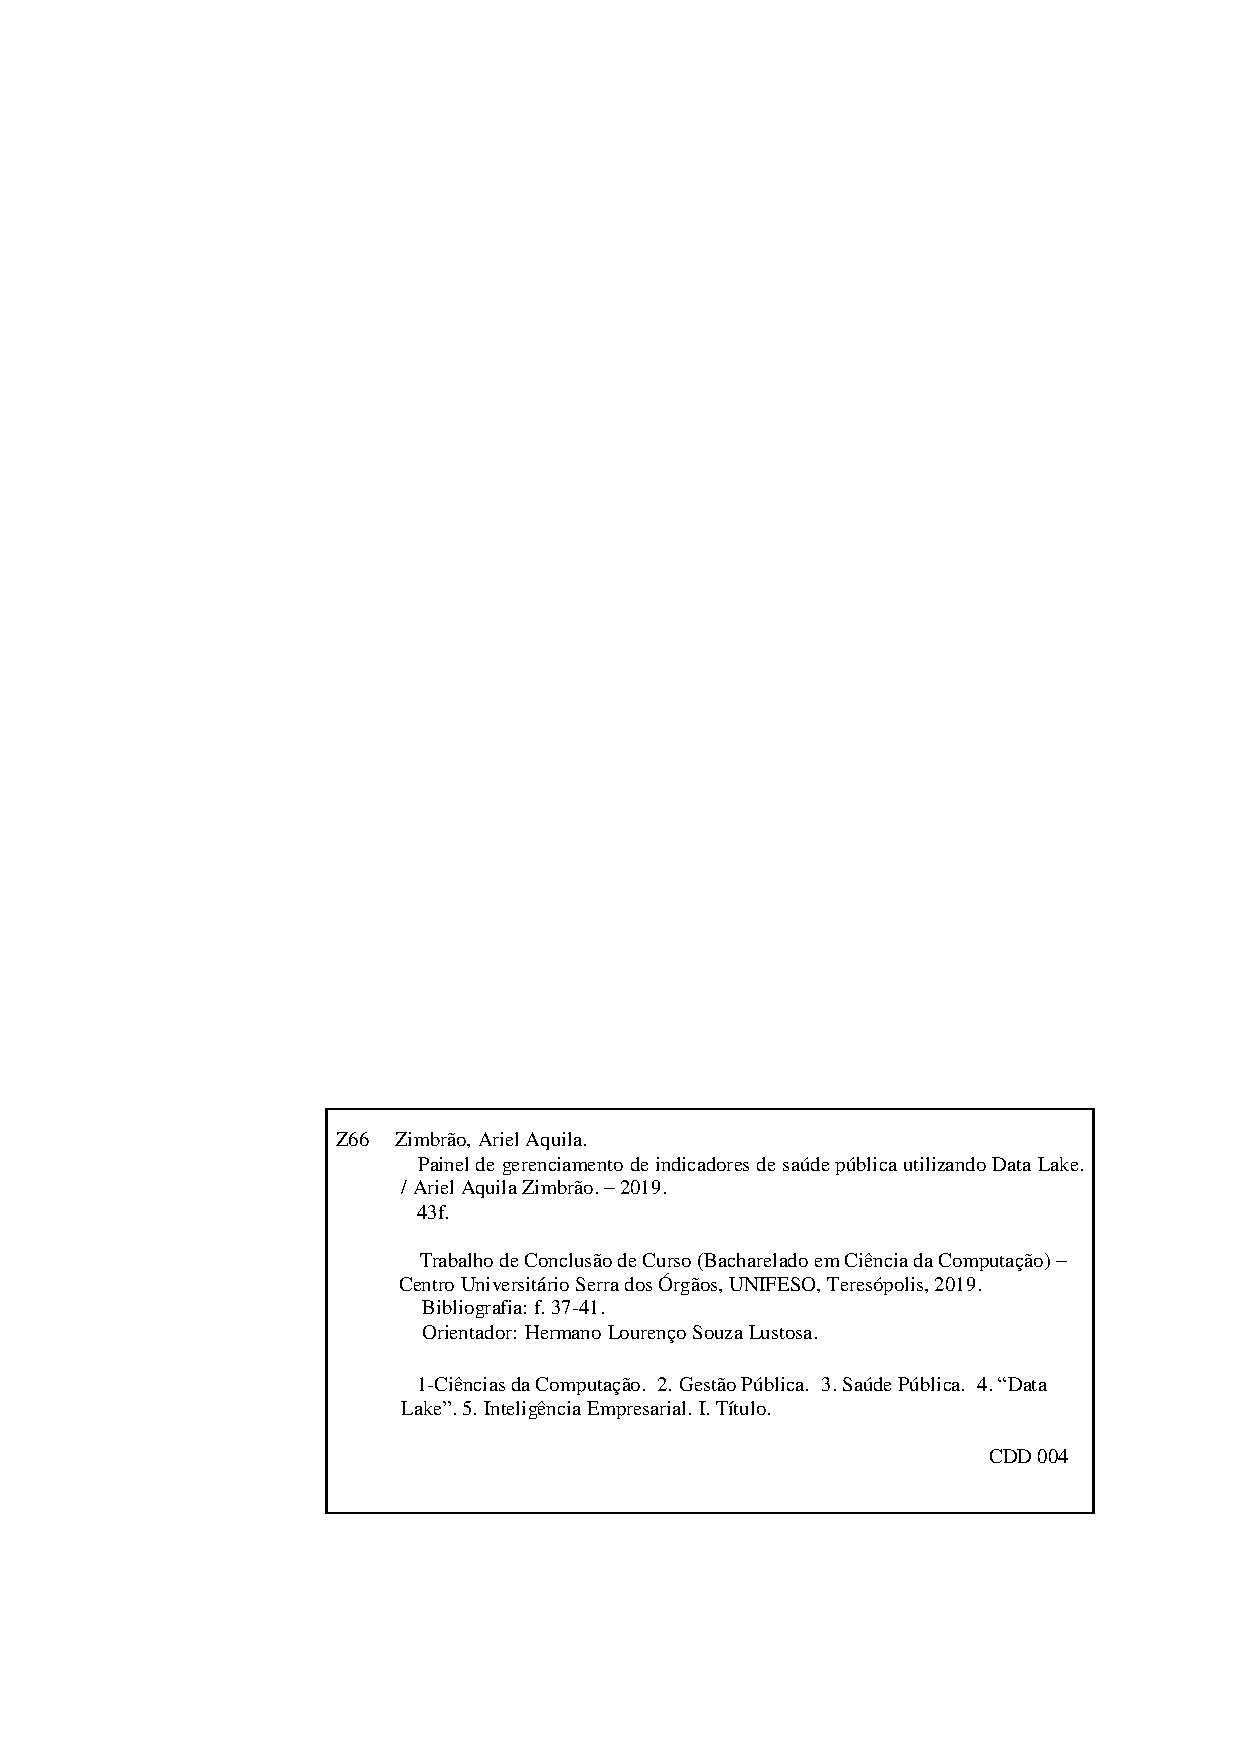
\includepdf{fichacatalografica.pdf}
\end{fichacatalografica}


\newpage
% ---
% ---

% ---
% Inserir folha de aprovação
% ---
%
\begin{folhadeaprovacao}
\imprimirfolhadeaprovacao
\end{folhadeaprovacao}


% ---

% ---
% Dedicatória
% ---

% ESCREVA A SUA DEDICATORIA A DEDICATORIA QUE SE ENCONTRA NO ARQUIVO E APENAS UM EXEMPLO. ESCOLHA A DEDICATORIA QUE MAIS LHE AGRADAR. LEMBRE-SE DE UTILIZAR AS '\\' PARA PULAR LINHAS

\begin{dedicatoria}
   \vspace*{\fill}
   \flushright
   %\noindent
   \textit{Este trabalho é dedicado a minha família e amigos\\
   que confiaram, apoiaram e me incentivaram na minha caminhada}
\end{dedicatoria}
% ---

% ---
% Agradecimentos
% ---
\begin{agradecimentos}

Agradeço a Deus que em toda a minha vida esteve ao meu lado. Agradeço também a todos os meus amigos e família que sempre acreditaram e me apoiaram nos meus sonhos.

\end{agradecimentos}
% ---

% ---
% Epígrafe
% ---

% ESCREVA A SUA EPÍGRAFE A MESMA QUE SE ENCONTRA NO ARQUIVO E APENAS UM EXEMPLO. ESCOLHA A EPÍGRAFE QUE MAIS LHE AGRADAR. LEMBRE-SE DE UTILIZAR AS '\\' PARA PULAR LINHAS

\begin{epigrafe}
    \vspace*{\fill}
	\begin{flushright}
		\textit{``Não importa o quão ruim a vida possa ser,\\
   há sempre alguma coisa que você pode fazer e ter sucesso.\\
   Enquanto há vida, há esperança.''\\
		(Stephen Hawking)}
	\end{flushright}
\end{epigrafe}
% ---

% ---
% RESUMOS
% ---


% ---

% ---
% inserir lista de ilustrações
% ---
% UTILIZE CASO HAJA FIGURAS NA MONOGRAFIAS. EM QUASO DE AUSENCIA DE FIGURAS COMENTAR COM AS 3 LINHAS DE CODIGOS UTILIZANDO O '%'.
\pdfbookmark[0]{\listfigurename}{lof}
\listoffigures*
\cleardoublepage
% ---

% ---
% inserir lista de quadros
% ---
% UTILIZE CASO HAJA QUADROS NA MONOGRAFIAS. EM QUASO DE AUSENCIA DE QUADROS COMENTAR COM AS 3 LINHAS DE CODIGOS UTILIZANDO O '%'.

%\pdfbookmark[0]{\listofquadrosname}{loq}
%\listofquadros*
%\cleardoublepage
% ---

% ---
% inserir lista de tabelas
% ---

% UTILIZE QUASE HAJA TABELAS NA MONOGRAFIAS. EM QUASO DE AUSENCIA DE TABELAS COMENTAR COM AS 3 LINHAS DE CODIGOS UTILIZANDO O '%'.

%\pdfbookmark[0]{\listtablename}{lot}
%\listoftables*
%\cleardoublepage
% ---

% ---
% inserir lista de algoritmos
% ---

% UTILIZE CASO HAJA ALGORITMOS NA MONOGRAFIAS. EM QUASO DE AUSENCIA DE ALGORITMOS COMENTAR COM AS 3 LINHAS DE CODIGOS UTILIZANDO O '%'.

%\pdfbookmark[0]{\listalgorithmcfname}{loa}
%\imprimirlistadealgoritmos
%\cleardoublepage
% ---

% ---
% inserir lista de abreviaturas e siglas
% ---
% DEVE SER PREENCHIDA A MÃO LEMBRE-SE DE MANTER EM ORDEM ALFABETICA.
\begin{siglas}
  \item[SUS] Sistema Único de Saúde
  \item[IBGE] Instituto Brasileiro de Geografia e Estatistica
  \item[BI] Business Intelligence
  \item[SQL] Structured Query Language
  \item[SGBD] Sistemas de Gestão de Base de Dados
  \item[Daas] Database as a service
  \item[ETL] Extraction, Transformation, Loading
  \item[COAP] Contrato organizativo da ação pública da saúde
  \item[BSA] Business Software Alliance
\end{siglas}
% ---

% ---
% inserir lista de símbolos
% ---
% DEVE SER PREENCHIDA A MÃO LEMBRE-SE DE MANTER EM ORDEM ALFABETICA.
%\begin{simbolos}
%  \item[$ \theta $] Letra grega maiúscula theta
%\end{simbolos}
% ---

% resumo em português
\setlength{\absparsep}{18pt} % ajusta o espaçamento dos parágrafos do resumo
\begin{resumo}

Hoje, no Brasil, o SUS (Sistema único de saúde) não possui ferramentas que permitam uma gestão unificada de todas as camadas e esferas governamentais envolvidas. Não existe um software e nem indicadores definidos para avaliar essa área tão crítica, tornando difícil para os governantes definir qual é a real situação da saúde pública brasileira.
O objetivo deste trabalho é desenvolver uma plataforma que forneça dados e indicadores sobre a saúde pública em cidades, estados e regiões do país, utilizando para isso uma estrutura simplificada de \textit{data lake} e dados de pesquisas fornecidos publicamente por instituições confiáveis. A ideia principal é fornecer uma ferramenta que auxilie na tomada de decisão do governo em ações direcionadas à área.

 \textbf{Palavras-chave}: \imprimirpalavraschave
\end{resumo}

% resumo em inglês
\begin{resumo}[Abstract]
 \begin{otherlanguage*}{english}
 
Today, in Brazil, the SUS (sistema único de saúde) has no tools that allows for the unified management of all levels and government spheres involved. There is no software and no defined indicators to evaluate this critical area, making it difficult for the rulers to define what is the real situation of the Brazilian public health.
The objective of this work is to develop a platform that provides data and indicators on public health in cities, states and regions of the country, using a simplified \textit{data lake} 
structure and research data provided publicly by trusted institutions. The main idea is 
to provide a tool that assists the governement in health related descision making.

   \vspace{\onelineskip}

   \noindent 
   \textbf{Keywords}: Public Management, Public Health, Data Lake, Business Intelligence.
 \end{otherlanguage*}
\end{resumo}

% ---
% inserir o sumario
% ---
\pdfbookmark[0]{\contentsname}{toc}
\tableofcontents*
\cleardoublepage
% ---



% ----------------------------------------------------------
% ELEMENTOS TEXTUAIS
% ----------------------------------------------------------
\textual
\pagestyle{simple}

% ----------------------------------------------------------
% Introdução
% ----------------------------------------------------------
\chapter{Introdução}

    O sistema único de saúde brasileiro, SUS, é um dos maiores e mais completos sistemas de saúde pública do mundo. Este programa tem como objetivo fornecer a toda população atendimento de saúde desde a atenção básica, como consultas para averiguação de pressão arterial ou glicose, a média e alta complexidade, como internações e transplantes de órgãos.
    
    O SUS possui 3 princípios organizacionais que modelam sua estrutura, sendo eles a regionalização, a descentralização e a participação popular (MINISTÉRIO DA SAÚDE, 2019). Tais princípios visam fornecer à população um serviço de melhor qualidade, mas também criam uma estrutura de gestão fracamente acoplada e de difícil fiscalização. O princípio da descentralização, por exemplo, divide a gestão da saúde pública entre os níveis de esfera governamental, o que causa um afastamento de discurso entre as instâncias superiores (estatual e federal) e a gestão municipal. Um exemplo simples é que se hoje um governador desejar criar um relatório relacionando o número de unidades básicas de saúde com o número de registro de turbeculose em cada cidade de seu estado,  ele necessitará que cada governo municipal colete e envie esses dados, através de suas secretarias de saúde, para o governo estadual, para que ele possa condensar em um único lugar as informações e assim montar relatórios. 
    
    A solução ideal para tal problema é a utilização, em âmbito nacional, de um sistema computacional que pudesse condensar as informações de todos os processos do SUS, servindo como fonte de dados a níveis micro e macro para os gestores públicos. Porém, tal solução é muito onerosa e necessitaria de um grande investimento financeiro por parte do governo, além de ser de difícil implantação dado o tamanho e o numero de municípios no Brasil. Já temos algumas ações a nível estadual que visam informatizar e integrar todas as entidades que compõe a saúde pública. Um exemplo é o estado do Paraná, que contratou um sistema de gestão de saúde pública de uma empresa privada e implantou em suas unidades de atendimento pelo SUS e com isso conseguiu realizar uma melhor gestão de recursos e serviços (MV informatiza sistema de saúde pública do Paraná, 2014).

    Uma outra solução possível é a utilização das fontes de dados confiáveis já publicamente disponíveis, como por exemplo, as pesquisas dos institutos IBGE (IBGE, 2019), Oswaldo Cruz (FIOCRUZ, 2019), Cruz vermelha (CRUZ VERMELHA, 2019), Ministério da Saúde (MINISTÉRIO DA SAÚDE, 2019) entre outros. Se essas informações fossem consolidadas em uma única estrutura, permitindo um consulta integrada aos dados, isto poderiam ser uma ferramenta útil para otimizar a gestão pública. Para o exemplo dado acima, podemos unir as pesquisas do IBGE que apresentam o número de unidades básicas de saúde em funcionamento por município com os registros do ministério da saúde que demostram o número de casos de turbeculose registrados por municípios, relacionados esses dados poderia verificar se um aumento no numero de unidades básicas de saúde reflete no número de casos de turbeculose. 
    
    Tal solução poderia se utilizar de tecnologias como \textit{data lake} (AWS - WHAT IS A DATA LAKE, 2019), Polystores (A. Dziedzic & A. J. Elmore, 2015),
    Daas (What is Database as a service, 2017) e entre outras, criando uma plataforma de BI (Business Intelligence) que apresente os dados consolidados de diversas fontes, permitindo também realização de filtro para a visualização dos dados a níveis municipal, estadual, regional e nacional.
    
    Sendo assim, esse trabalho visa utilizar de uma estrutura simples de \textit{data lake} para criar uma plataforma de BI que consolide diversas fontes de
    dados sobre a área da saúde, tendo como objetivo desenvolver um protótipo de ferramenta que poderá ser utilizado por gestores públicos para o auxílio a tomada de decisão.
    
    No trabalho proposto, foram desenvolvidos painéis para análise de dados que permitem relacionar dados oriundos de distintas fontes e formatos, conforme descrito na Secão 3.2 desse trabalho, a partir de uma estrutura simples de \textit{data lake}, possibilitando uma análise de dados integrada.
    
    Este trabalho está organizado da seguinte forma: o capítulo dois aborda a fundamentação teórica, onde será exposto um pouco mais sobre todas as tecnologias e conceitos que norteiam o projeto. O capítulo três refere-se à metodologia, expondo as ferramentas e dados utilizados para a realização do trabalho proposto. No capítulo quatro é apresentado o processo de desenvolvimento do projeto e suas etapas. O quinto capítulo apresenta as conclusões, resultados obtidos e propostas para projetos futuros. 

\chapter{Fundamentação Teórica}
    Neste capitulo será apresentado alguns dos princípios teórico que deram base para o desenvolvimento desse projeto, como funciona a gestão da saúde pública no Brasil e conceitos sobre banco de dados,\textit{bussiness intelligence} e \textit{data lake}. 
    
\section{Gestão de Saúde Pública}

    Para se propor uma solução na área de saúde pública é necessário entender como ela está estruturada e quais são seus pontos fortes e fracos. O SUS (sistema único de saúde) é um dos mais completos e abrangentes sistemas de saúde pública do mundo. Sua abrangência vai desde a atenção básica, média e alta complexidade, até serviços de urgência, vigilância epidemiológica e entre outros (MINISTÉRIO DA SAÚDE, 2019).
    O SUS possui 6 princípios divididos em princípios ideológicos e organizacionais. Os princípios ideológicos se referem a ideologia que norteia as decisões estratégicas do programa, e são elas a:
    \begin{description}[font=$\bullet$~\normalfont\scshape\color{black!50!black}]
    \item [Universalidade] diz que todo o cidadão tem direito ao SUS independente de quem seja;
    \item [Equidade] garante a universalidade considerando as diferenças, dedicando mais esforço onde é necessário; e 
    \item [Integridade] que visualiza o cidadão como um todo fornecendo a ele todos os níveis de atenção a saúde.
    \end{description}
    Os princípios organizacionais definem a forma como a estrutura do programa deve ser moldada e gerenciada, e são eles a:
    \begin{description}[font=$\bullet$~\normalfont\scshape\color{black!50!black}]
    \item [Descentralização] que divide a gestão do sistema único de saúde entre os níveis do governo;
    \item [Regionalização/Hierarquização] que diz que os serviços devem ser organizados pelo nível de complexidade, levando em consideração as variações e características regionais; e 
    \item [Participação Popular] que institui a criação de conselhos e conferências de saúde, visando trazer a população para o dia a dia do sistema.
    \end{description}
    (LEGISLAÇÃO DO SUS, 2019) (MINISTÉRIO DA SAÚDE, 2019) 
    
    Devido ao princípio da descentralização, cada esfera do governo tem responsabilidades sobre o sistema, sendo elas autônomas e soberanas sobre suas decisões e atividades. Cada esfera do governo também possui entidades anexadas para a realização das tarefas associadas a ela, como mostrado na Figura \ref{Esferas do governo e suas entidades}. A união, atuando através do ministério da saúde, tem como papel ser o principal financiador do SUS, mas também tem a função de elaborar normas e instrumentos de controle além de avaliar o sistema. Os governos estaduais e do distrito federal são responsáveis pela gestão da saúde em seu território. Eles devem aplicar fundos próprios além de repassar para os municípios as verbas destinadas a saúde oriundas da união e também podem criar políticas próprias, mas devem obedecer às normalizações do governo federal. Os municípios têm como responsabilidade executar ações e serviços de saúde em seus respectivos territórios. Os municípios podem aplicar fundos próprios, porém também recebem verbas para aplicar na saúde, vindas dos governos estaduais e do governo federal. (MINISTÉRIO DA SAÚDE, 2019).
    
    \begin{figure}[H]
         \centering
         \caption{Esferas do governo e suas entidades}
         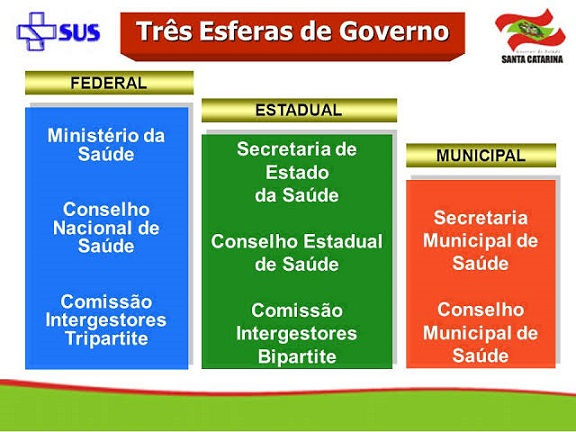
\includegraphics[scale=1]{imagens/esferas-entidades.jpg}
         \\{\footnotesize Fonte: 5° ENCONTRO DE GESTORES MUNICIPAIS DE SAÚDE MODELO DE GESTÃO - SANTA CATARINA, 2014}
         \label{Esferas do governo e suas entidades}
    \end{figure}
    

\section{Sql e NoSql}

    SQL (Structured Query Language) é uma linguagem de consulta que é utilizada em bancos de dados relacionais. O termo SQL também pode ser utilizado para definir este tipo de estrutura para banco de dados em oposição ao termo NoSQL, que define estruturas de banco de
    dados não relacionais. Os bancos de dados relacionais armazenam os dados em tabelas, como mostrado na Figura \ref{exemplo tabela}, onde um dado armazenado em uma coluna de uma tabela pode indicar um item em outra tabela, criando assim uma relação entre elas. Exemplos de SGBD (Sistema de gerenciamento de banco de dados) que trabalham com banco de dados relacional são o PostgreSQL (PostgreSQL, 2019), Oracle (Banco de dados - Oracle, 2019), SQL Server (Plataforma de Dados da Microsoft, 2019) entre outros. 
    
    \begin{figure}[!h]
         \centering
         \caption{Exemplo de tabela de um banco de dados relacional}
         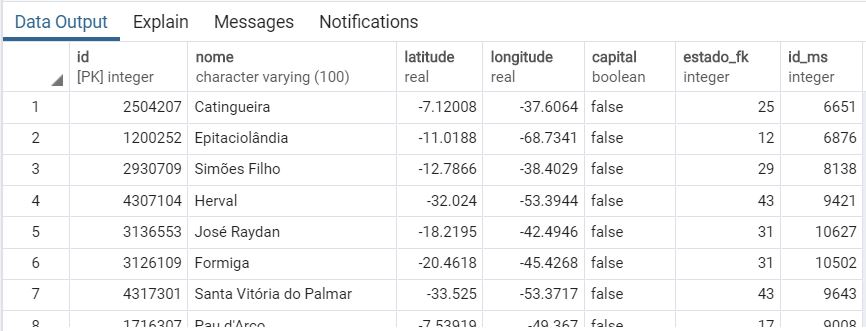
\includegraphics[scale=0.8]{imagens/exemplo-tabela.jpg}
         \\{\footnotesize Fonte: Produção do próprio autor utilizando a plataforma PostegreSQL}
         \label{exemplo tabela}
    \end{figure}

    Com a linguagem SQL podemos criar e manipular banco de dados relacionais. Ela possui uma sintaxe simples que visa se aproximar da fala humana, o que facilita a aprendizagem e o entendimento de scripts em SQL. Apesar do SQL possuir um conjunto de comandos comuns a todos os bancos de dados relacionais, cada banco pode implementar comandos extras que tem como objetivo facilitar o desenvolvimento.

    O termo NoSQL se refere ao conjunto de sistemas de banco de dados que não possui uma estrutura de tabelas relacionais. Dentro do NoSql possuímos uma gama imensa de diversas formas de armazenar, representar e consumir os dados, cada qual possuindo sua aplicação.
    
    Um exemplo de um banco de dados NoSQL é o MongoDB (MongoDB - The most popular
    database for morden apps, 2019). O MongoDB possui uma estrutura baseada em documentos. Nele podemos armazenar os dados em formato de objeto, como mostrado na Figura \ref{exemplo objeto}. No MongoDB, no lugar de utilizamos consultas em SQL para manipular os dados, é utilizado o MQL (MongoDB Query Language), e com ela podemos inserir, deletar, atualizar e consultar dados. 
    
    \begin{figure}[H]
         \centering
         \caption{Exemplo de dado em formato de objeto}
         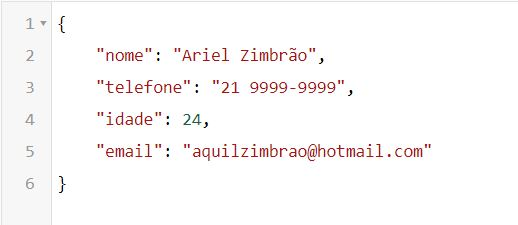
\includegraphics[scale=1]{imagens/objeto.JPG}
         \\{\footnotesize Fonte: Produção do próprio autor}
         \label{exemplo objeto}
    \end{figure}
    
    No MongoDB, as consultas são feitas pelos valores contidos dentro dos objetos que estão armazenado em seu banco, como podemos ver na Figura \ref{exemplo query mongo}.
    
    \begin{figure}[H]
         \centering
         \caption{Exemplo de consulta em MQL}
         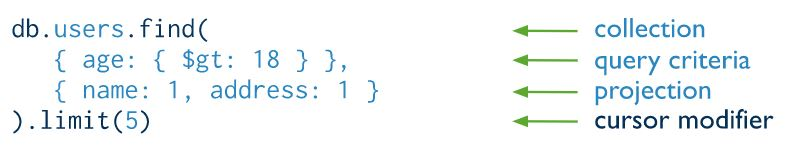
\includegraphics[scale=1]{imagens/mongo-query-exemplo.JPG}
         \\{\footnotesize Fonte: (MongoDB CRUD Operations - MongoDB Manual, 2019)}
         \label{exemplo query mongo}
    \end{figure}
    
    Um outro exemplo de banco de dados muito utilizado é o Redis (Redis, 2019). O Redis é um banco de dados baseado na arquitetura chave-valor. No Redis, podemos armazenar qualquer tipo de dado, porém é necessário sempre definir uma chave, um nome para esse dado. As consultas são feitas com a utilização da chave que foi definida. O Redis é muito utilizado para armazenamento de dados temporários em aplicações web e mobile. Tal arquitetura possui como principal vantagem possuir consultas muito rápidas. Os comandos mais básicos do Redis são: GET e SET, que podem ser vistos na Figura \ref{exemplo comandos redis}.
    
    \begin{figure}[H]
         \centering
         \caption{Exemplo de comandos redis}
         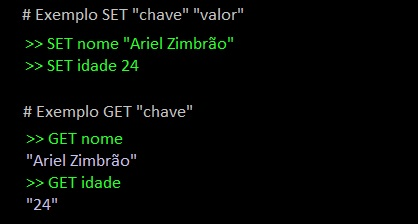
\includegraphics[scale=1]{imagens/exemplo-redis.JPG}
         \\{\footnotesize Fonte: Produção do próprio autor}
         \label{exemplo comandos redis}
    \end{figure}
    
    Também temos o InfluxDB (InfluxDB - Porpuse-Built Open Source Time Series DataBase, 2019), que é um SGBD NoSQL de série temporal, ou seja, os dados no InfluxDB têm  como principal índice a data da ocorrência. Este SGBD é muito utilizado para análise de dados históricos, normalmente conectados a outras plataformas que permitem a visualização dos dados em tempo real, como por exemplo, o Grafana (Grafana - The open observability platform, 2019). Uma aplicação muito comum para o InfluxDB junto 
    ao Grafana é para o monitoramento de aplicações em tempo real, ou seja, podemos utilizar tais tecnologias para o monitoramento, em tempo real de serviço online, utilizando o InfluxDB para armazenar as informações e o Grafana como painel de visualização, de dados como freguência de acesso, tempo online e etc, da mesma forma que pode ser visto na Figura \ref{influxdb com grafana}.

    \begin{figure}[H]
         \centering
         \caption{Painel Grafana utilizando InfluxDB}
         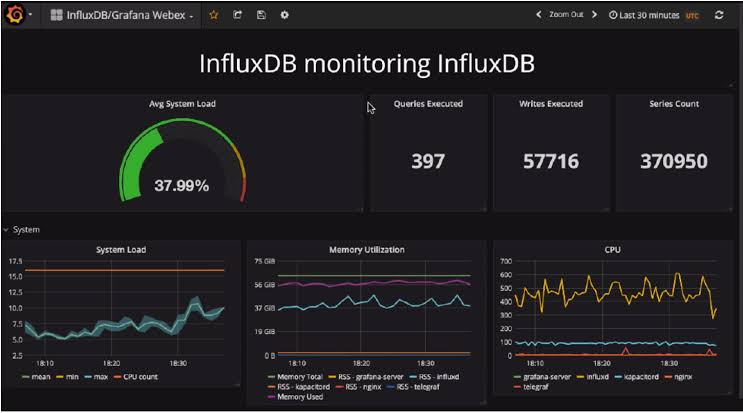
\includegraphics[scale=0.5]{imagens/influx-grafana.jpg}
         \\{\footnotesize Fonte: (InfluxDB Time Series Data Monitoring With Grafana, 2019)}
         \label{influxdb com grafana}
    \end{figure}
\section{DaaS (Database as a Service)}
    
    DaaS significa "Database as a Service", ou traduzindo, "Banco de dados como serviço". Este é um modelo de serviço que vem crescendo a cada dia e oferece diversas vantagens aos seus usuários. Empresas como a Amazon (AWS - Amazon Web Services, 2019) e Google (Google Cloud, 2019) já possuem serviços de computação em nuvem, não somente para hospedagem de banco de dados, mas também para controle e manutenção, além de oferecer uma gama de ferramentas que podem ser utilizadas para realizar análises sobre os dados armazenados em um database.

    O Google e a Amazon de longe são as empresas de referência quando falamos em computação em nuvem e ciência de dados. Ambas possuem diversos serviços, como por exemplo o Google Cloud Dataflow (Google Cloud Dataflow, 2019) e o Amazon Athena (Amazon Athena, 2019) que são ferramentas Daas que permitem a realização de transformação e consulta de dados respectivamente, e são plataformas que podem ser acessadas a qualquer momento via internet.
    
    A grande vantagem em utilizar sistemas DaaS é sua escalabilidade. A escalabilidade é a capacidade de aumentar de tamanho mantendo desempenho adequado. Isto é uma característica desejável a bancos de dados, porém há muita dificuldade em prover tal característica, o que faz problemas de escalabilidade ser algo comum relacionado a bancos de dados
    Um conhecido problema relacionado a banco de dados é como escalar um banco, ou seja aumentar um banco de dados. Plataformas como o Google Cloud e a Amazon Web Service já contém recursos que nos permite resolver esses problemas conhecidos com alguns cliques, agilizando muito o desenvolvimento de qualquer projeto. Porém, dependendo do tipo de projeto, a utilização de plataformas DaaS pode se tornar cara, sendo melhor se o projeto não precisar de alta disponibilidade, como alocar os seus serviços de banco de dados localmente.
    
\section{BI - Bussiness Intelligence}

    O termo Business Intelligence, ou BI, refere-se à tecnologia que visa coletar, armazenar, analisar e apresentar dados referentes ao negócio (What is Business Intelligence (BI)?, 2019). Tendo como objetivo ajudar as empresas e instituições nas tomadas de decisões mais assertivas, visa demonstrar os dados de forma consolidada em relatórios.
    
    Para se montar um BI, em seu modelo mais tradicional, alguns passos são necessários. como podemos ver na Figura \ref{construcao de bi}. O primeiro passo é analisar e conhecer os dados. Esta etapa é muito importante, pois a coerência e integridade dos dados são muito importantes no BI. A segunda etapa na criação de uma
    plataforma de Bussiness Intelligence é a consolidação dos dados, isto é, a extração dos dados de sua fonte original à conversão ou transformação dos mesmos e depois o seu armazenamento de forma organizada a um banco de dados relacional - banco este que é denominado \textit{DataWarehouse} (Armazém de dados). Este processo é denominado ETL (Extraction, transformation, loading), no final criamos os painéis de visualização, ou seja gráfico que consigo mostrar os dados de forma a facilitar a extração de informações e agregar valor ao négocio. 
    
    Hoje, já existem no mercado diversas ferramentas que podem nos auxiliar no trabalho de consolidação de dados, como por exemplo o SQL Server Data Tools (SQL Server Data Tools, 2017), que é uma ferramenta que trabalha integrada ao banco de dados SQL Server (Plataforma de Dados da Microsoft, 2019) e permite a realização de ETL diretamente pela interface do SGBD. Também existem soluções no modelo Daas (Database as a service), como por exemplo o Google Cloud Dataflow (Google Cloud Dataflow, 2019) que realiza toda a transformação e consolidação dos dados em uma plataforma web. Também existem soluções no modelo Daas (Database as a service), como por exemplo o Google Cloud Dataflow (Google Cloud Dataflow, 2019) que realiza toda a transformação e consolidação dos dados em uma plataforma web. Depois de processados e consolidados em um DW (DataWarehouse), tais informações precisam ser expostas de uma forma clara para qualquer pessoa, e isto normalmente é feito utilizando os dados armazenados no DW para se criar painéis contendo gráficos interativos. Para tal tarefa, existem algumas ferramentas que podem nos auxiliar, como por exemplo o Qlik (Análise de dados para o Business Intelligence moderno, 2019), Tableau (Tableau - Software de análise e bussiness intelligence, 2019) ou o Power BI (Power BI - Ferramentas do BI de Visualização de dados Interativa, 2019). Os painéis criados por estas ferramentas são de fácil entendimento e manipulação.
    
    \begin{figure}[H]
         \centering
         \caption{Etapas da criação de um BI}
         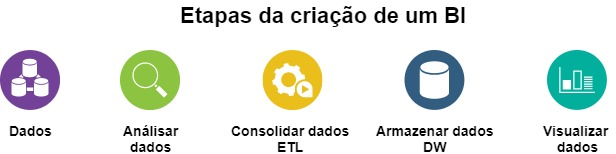
\includegraphics[scale=0.6]{imagens/criacao-bi.jpg}
         \\{\footnotesize Fonte: Produção do próprio autor}
         \label{construcao de bi}
    \end{figure}
    
    As plataforma de suporte para visualização de dados de BI como o Qlik utilizam de um estrutura interna chamada de OLAP que significa \textit{On-Line Analytical Processing} ou, traduzindo, processamento analítico online, isso significa que o dado não é armazenado em uma estrutura de tabelas tendo agora uma estrutura virtual que se assemelha a um cubo formado de diversos outro cubos, como podemos ver na Figura \ref{estrutura olap}. Também podemos ver nessa figura algumas das alterações possíveis de um OLAP como \textit{roll up}, \textit{drill down} e \textit{dicing}, essas operações possibilitam a existência de recursos muito comuns em painéis de BI, como filtros e níveis de visualização. Um exemplo é se um usuários estiver visualizando o número de casos de um doença por municípios e desejar agrupar esse dados para visualizar a nível de estado ele estará realizando uma operação de \textit{roll up}, se retornar a visualização de município ele estará realizando um \textit{drill down} e se ele desejar filtrar somente os municípios de um estado, ele estará realizando uma operação de \textit{dicing}.
    
    \begin{figure}[H]
         \centering
         \caption{Estrutura olap}
         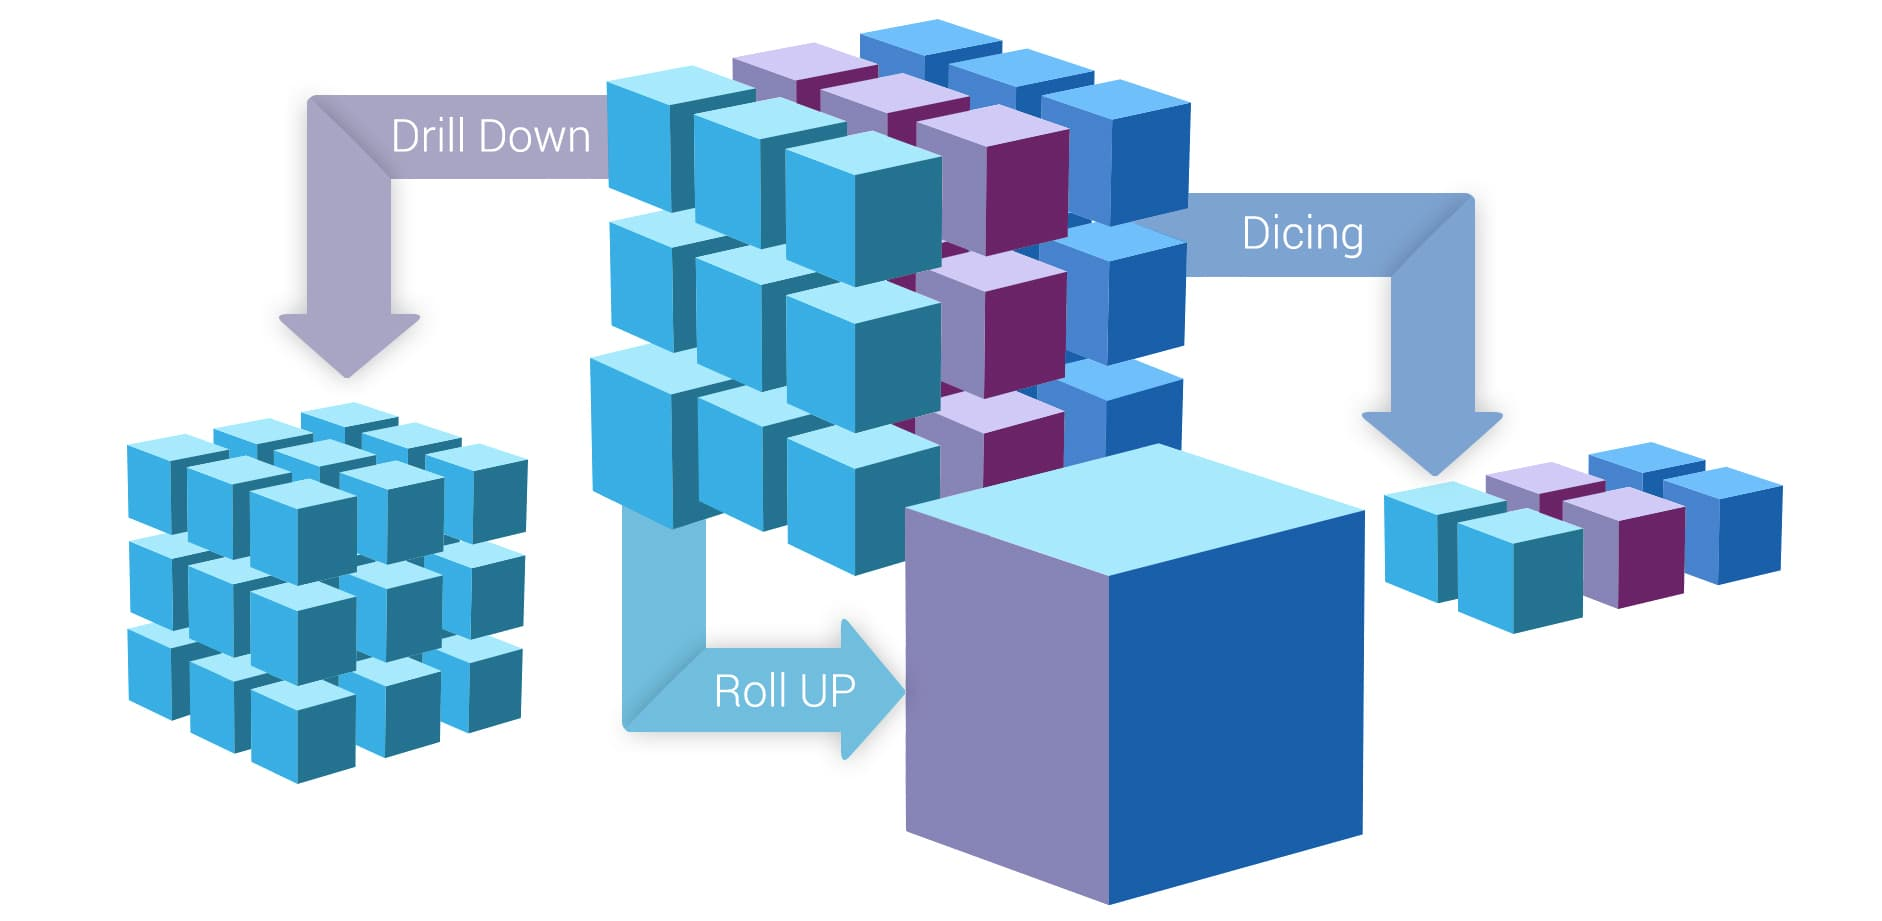
\includegraphics[scale=0.2]{imagens/olap_operations.jpg}
         \\{\footnotesize Fonte: The Technology of an OLAP Cube, 2019}
         \label{estrutura olap}
    \end{figure}
    
    
\section{Data Lake}

    \textit{Data lake} é uma estrutura  que permite armazenar, em um único repositório centralizado, dados de diferentes tipos e fontes, dando estrutura para a realização de consultas e análise de dados. (AWS - WHAT IS A DATA LAKE, 2019). Com um \textit{data lake}, ou lago de dados, podemos ter dados de diferentes formatos em um único lugar, possibilitando que análises sejam realizadas a partir destes dados.
    No modelo tradicional de BI (Business Intelligence), todos os dados deveriam passar por uma etapa de processamento para serem consolidados em um \textit{DataWarehouse}, e a partir daí, serem úteis para análise. Um \textit{DataWarehouse} é um banco de dados relacional onde é inserido de forma consolidada os dados para uma posterior análise dentro de um modelo convencional de \textit{Business Intelligence}. Já com o \textit{data lake}, podemos trabalhar sobre os dados em seu formato inicial, o que evita uma possível perda de informação que possa ser gerada em um processamento, além de dar a possibilidade de trabalhar com os dados em tempo real. 
    
    O \textit{data lake} é apenas um conceito, ou seja, existem diferentes formas de se implementar uma estrutura de \textit{data lake}, porém alguns pontos precisam ser observados para não tornar o seu lago de dados em um pântano, ou \textit{data swamp}, como é chamado estruturas de \textit{data lake} mal projetadas. 
    
    Um dos pontos que precisam de atenção na criação e manutenção de um \textit{data lake} são os metadados. Metadados são utilizados para classificar e organizar os dados armazenados. Os metadados dão informações sobre a semântica do dado e isso ajuda e definir, por exemplo, como esse dados serão utilizados, quem tem interesse nele e por quanto tempo ele deve ser exposto (Information Age - The difference between a \textit{data swamp} and a \textit{data lake}? 5 signs, 2019). A estrutura de uma \textit{data lake} é divida em camadas, como podemos ver na Figura \ref{Estrutura data lake},  não há um número máximo de camadas para a implementação de um \textit{data lake}, pois tal estrutura pode ser moldada e possui mais ou menos camadas, dependendo da necessidade.
    
    \begin{figure}[H]
         \centering
         \caption{Estrutura básica de um \textit{data lake}}
         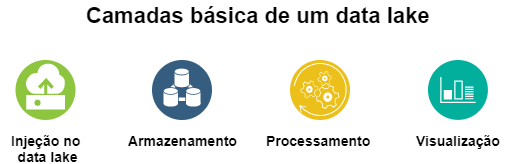
\includegraphics[scale=0.8]{imagens/estrutura-datalake.png}
         \\{\footnotesize Fonte: Produção do próprio autor utilizando a plataforma Draw.io}
         \label{Estrutura data lake}
    \end{figure}
    
   Grandes empresas que fornecem serviços tecnológicos, em especial na computação em nuvem, como a Amazon AWS (Amazon Web Service, 2019) e o Google (Google Cloud, 2019), estão trabalhando em ferramentas para a área das ciências de dados. Em ambas as plataformas, o usuário consegue montar uma estrutura inteira de \textit{data lake} totalmente na nuvem usando ferramentas como o S3 e o Athenas da Amazon ou o \textit{DataFlow} e o \textit{BigQuery} do Google.

    O grande desafio de criar e manter um \textit{data lake} é garantir a coerência dos seus dados contidos na estrutura no decorrer do tempo. Um \textit{data lake} aceita qualquer tipo de dado, porém nem sempre todos os dados de um negócio são úteis para integrar um \textit{data lake}. Tal análise cabe aos cientistas de dados responsáveis por sua estrutura. 
    
    Apesar de existirem diversas ferramentas e plataformas que auxiliem na criação e manutenção de um \textit{data lake}, como citado acima, um computador ainda não consegue entender qual é a semântica de um dado para então definir a sua relevância para o negócio. 
    
    Um exemplo simples sobre como é importante o estudo cuidadoso sobre os dados que serão inseridos em um \textit{data lake} é uma empresa que está implementando o seu \textit{data lake}. Existem duas planilhas que contém a informação de satisfação do cliente, mas uma está medindo a satisfação com notas de 0 a 10 e outra com notas de 0 a 5. Neste caso, temos dois dados que nos dão a mesma informação, com isso, manter os dois dados no \textit{data lake} apenas deixaria ele mais pesado e não iria agregar valor, sendo o correto, verificar com os gestores da empresa qual é a melhor visualização e manter somente um dado referente a satisfação do cliente.
 
    Apesar de todos os desafios de se criar e manter um \textit{data lake}, existem empresas, inclusive brasileiras, que estão investindo nessa tecnologia, pois viram no \textit{data lake} uma forma de extrair de um monte de dados valor para o seu negócio. Um exemplo disso é a Movile, uma empresa líder na América Latina em marketing place mobile, possuindo grande marcas conhecidas como IFood, PlayKids entre outros (Movile - O Grupo, 2019). 
    
    O Movile trabalha em diversos projetos e com isso houve a necessidade de se criar um \textit{data lake} para integrar os diversos dados em um único ambiente. Depois de muito analisar, os engenheiros da Movile montaram uma estrutura de \textit{data lake} utilizando tecnologias em nuvem, como Google Cloud Storage (Google Cloud Storage, 2019), Google BigQuery (Google Cloud BigQuery, 2019), Presto (Presto - Distributed SQL Query Engine for Big Data, 2019), Amazon S3 (Amazon S3, 2019), Amazon Athena (Amazon Athena, 2019) e Amazon Redshift Spectrum (Amazon Redshift, 2019). (A jornada para implementação de um Data Lake, 2017). 
    
    Uma outra empresa brasileira que começou a investir em \textit{data lake}, dessa vez na área de saúde, é a \textit{Funcional Health Tech} (Funcional Health Tech, 2019), que é uma startup focada em gestão de saúde e análise de dados, que junto com a Globalweb (Globalweb - Uma nuvem de soluções para sua empresa, 2019), que é uma empresa que fornece serviço de computação em nuvem, estão desenvolvendo um \textit{data lake} que tem como funcionalidade aumentar a capacidade de gerar análise de dados integradas a tecnologias de aprendizagem de máquina. (IstoÉ Dinheiro, Funcional Health Tech investe em big data para a saúde, 2019) (Convergencia Digital, Globalweb desenvolve Data Lake para a Healthtech, 2018)
    
    O BI tradicional e a abordagem utilizando  \textit{data lake} possui aplicações diferentes. As vantagens de um \textit{data lake} são melhores aproveitadas se tenho um cenário com grande volume de dados e os mesmos são muito heterogênicos quanto ao formato e origem, como por exemplo em uma corporação que é formada por diversas outras empresas de ramos distintos. Na estrutura tradicional de um BI é necessário consolidar os dados em um único banco relacional que é denominado \textit{datawarehouse}, com isso a existência de um grande volume de dados distribuído em diversas fontes e formatos toram a criação e manutenção desse banco muito complexa. Na Figura \ref{diferenca bi datalake} podemos ver a diferença no processo de criação de um BI em sua estrutura tradicional, utilizando um \textit{datawarehouse}, e uma estrutura de \textit{data lake}. Podemos ver a existência de etapas em comum, porém podemos ver que as principais diferenças são em como os dados são armazenados. 
    
    \begin{figure}[H]
         \centering
         \caption{Diferença BI "tradicional vs"\textit{data lake}}
         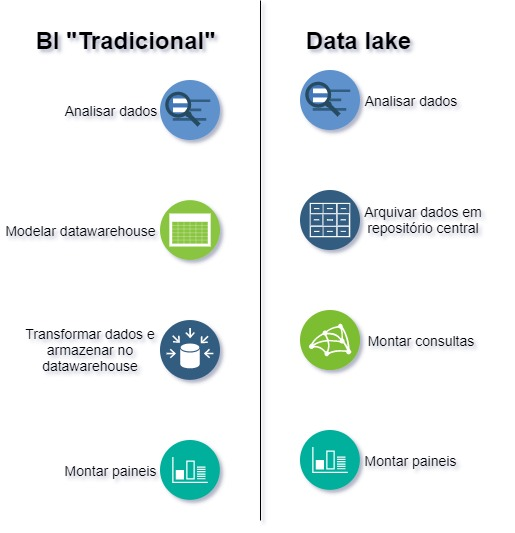
\includegraphics[scale=0.7]{imagens/bi_x_datalake.jpg}
         \\{\footnotesize Fonte: Produção do próprio autor}
         \label{diferenca bi datalake}
    \end{figure}

\chapter{Metodologia}
    
    Este trabalho tem como objetivo utilizar de uma estrutura de \textit{data lake} e dados de pesquisas publicamente disponíveis em diversos formatos para criar um painel que apresente, de forma consolidada, dados da área da saúde, visando que tal plataforma possa auxiliar a tomada de decisão.
    Para isto foi necessário dedicar um tempo para estudo e aprofundamento na área de negócio proposta, entendendo como funciona o sistema único de saúde, SUS, sua organização e forma de gestão, descobrindo quais são as qualidades e pontos de melhoria do modelo de gestão escolhido para esse sistema. 
    
    Durante o desenvolvimento foram analisados algumas propostas que se assemelham a proposta deste trabalho, como por exemplo o COAP (contrato organizativo da ação pública da saúde) e o GovData. O COAP foi criado através de uma lei complementar do SUS e ele estabelece um acordo colaborativo entre todas as esferas do governo. O COAP é um documento, que quando aderido por uma determinada região de saúde, estabelece responsabilidades e métricas claras para a saúde publica, auxiliando na questão do sistema único de saúde.. (Secretária Estadual de Saúde de Pernambuco, Nota Técnica Número 6 - Orientações COAP, 2013) (Ministério da saúde, Contrato Organizativo de Ação Pública da Saúde, 2019). O GovData é uma plataforma de análise de dados públicos que utiliza de um \textit{data lake} integrando dados governamentais, com o foco em relacionar e coletar dados financeiros do governos,  como a distribuição de verbas para municípios, gasto com obras e etc. O GovData já possui alguns painéis de visualização de dados disponíveis publicamente. (GovData - Plataforma de análise de dados, 2019)
    
    Também foi realizado um estudo referente as tecnologias relacionadas a \textit{data lake} e as fontes de dados, ou seja, pesquisas relacionadas a área de saúde que estavam disponíveis publicamente. A partir desse estudo, foi definido o ferramental que foi utilizada no desenvolvimento desse trabalho. 
    
\section{Ferramentas}
    Aqui será apresentado as ferramentas que foram utilizadas no desenvolvimento desse projeto e os motivos que levaram a seleção das mesmas. 
    
\subsection{Python}
    
    O Python é uma linguagem de programação de alto nível e multi paradigmas criada em 1991 e mantida hoje em dia pela Python Software Foundation (About Python, 2019). 
    
    A linguagem Python é conhecida por ser uma linguagem de fácil aprendizagem, isso se dá principalmente a algumas características como a tipagem dinâmica, seu grande repositório de bibliotecas e o fato de ser uma linguagem interpretada. Atualmente com a evolução da tecnologia e o crescimento da ciência de dados, área focada no estudo e análise de dados, o Python vem ganhando muita popularidade, principalmente pela sua facilidade de tratar e transforma dados. Um outro fator que vem aumentando o número de adeptos ao Python e tem tornando a linguagem cada vez mais conhecida é o crescimento do aprendizado de máquina. Em novembro de 2015, a Google lançou o TensorFlow, que é uma biblioteca em Python para a criação de sistema de aprendizagem de máquina (Why TersonFlow, 2019), que ficou muito conhecida, trazendo um aumento significativo da comunidade de usuários de Python (Python mantém ascenção e ganha ainda mais popularidade, 2019). 
    
    Neste projeto o Python foi utilizado na sua versão 3.6  na etapa na preparação dos dados, veja seção 4.4, visando tratar os dados e permitir o relacionamento entre eles. O Python foi escolhido por ser uma linguagem de programação muito utilizada para análise de dados, por ser de fácil aprendizagem.
    
        
\subsection{Dremio}

    O Dremio (Dremio is the \textit{data lake} engine, 2019) é uma plataforma DaaS (Database as a Service) que permite conectar diversas fontes de dados, de diferentes formatos, e consumí-las, utilizando comandos em SQL. Neste trabalho, o Dremio será mecanismo responsável por agregar nossos dados e fornecer um meio rápido de acessá-los.

    O Dremio foi escolhido por ser uma solução única que agrega diversas funções ao \textit{data lake}, sendo elas o armazenamento, categorização, conexão e consumos dos dados, simplificando a estrutura necessária para se atingir os objetivos deste projeto. 
    
    O Dremio também é utilizado como camada de agregação de dados em  \textit{data Lakes} mais complexos, pois ele pode ser utilizado conectado a outros serviços, como por exemplo: as soluções da AWS (Amazon Web Service, 2019), para \textit{data lake}.
    
    \begin{figure}[H]
         \centering
         \caption{Tela de montagem de query no Dremio}
         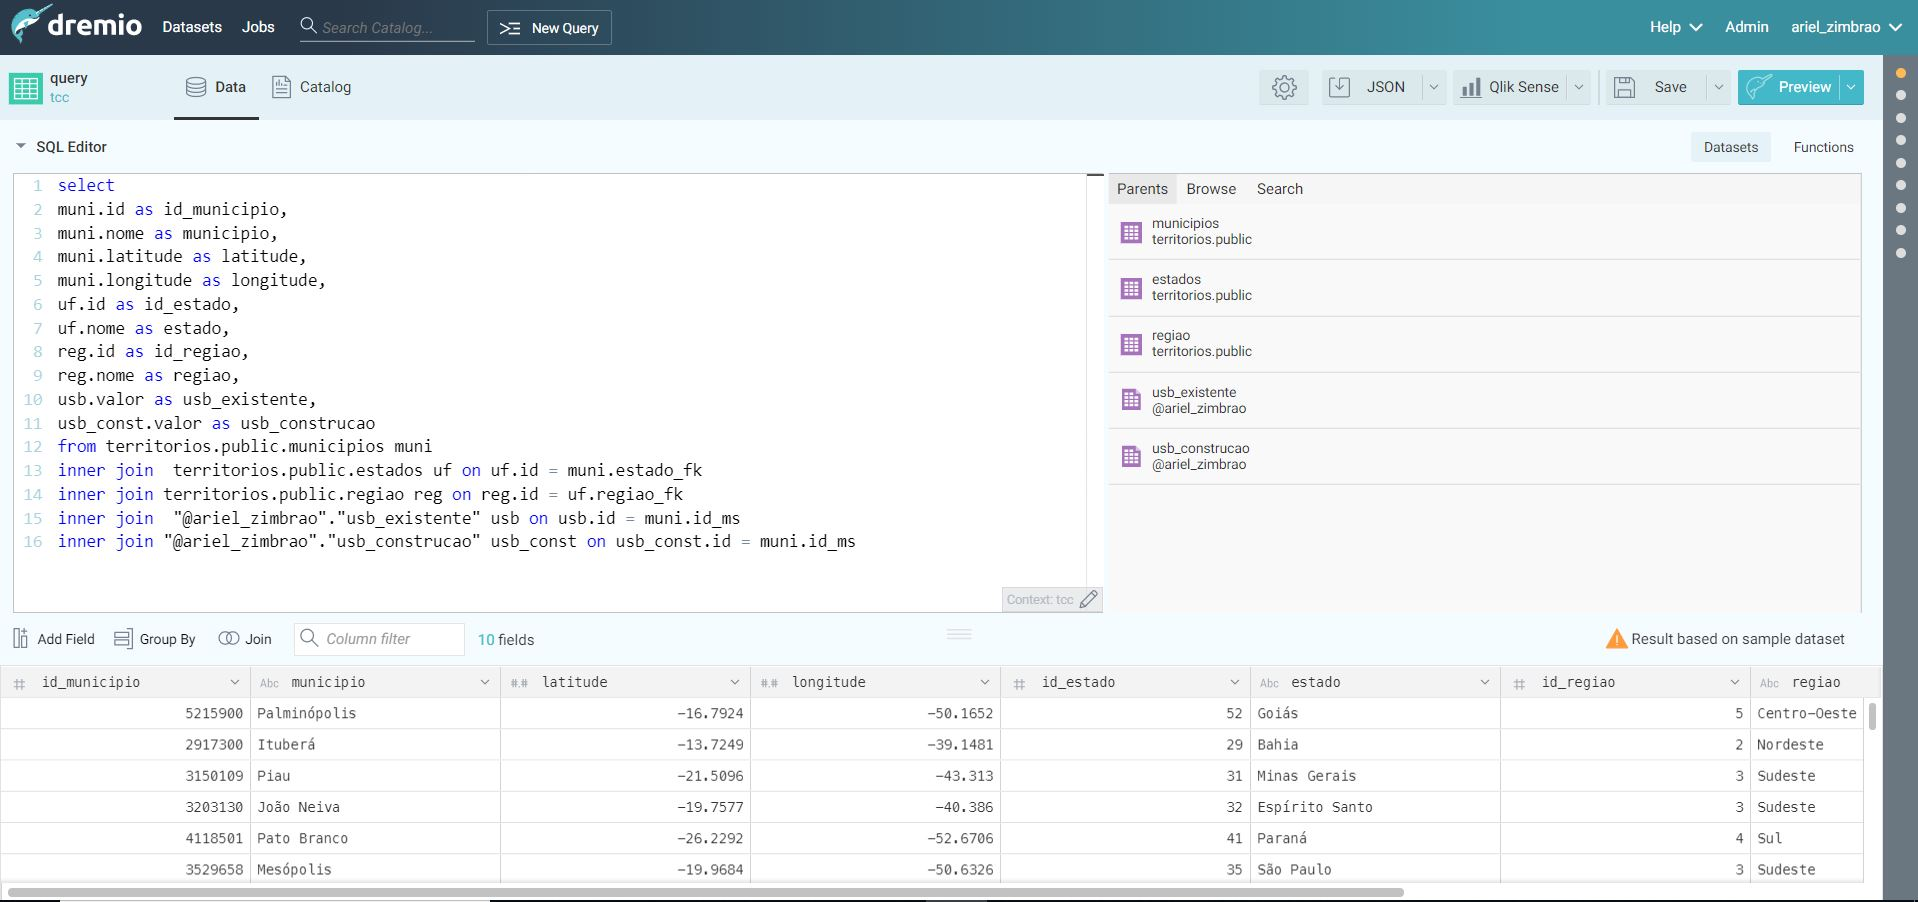
\includegraphics[scale=0.4]{imagens/dremio.JPG}
         \\{\footnotesize Fonte: Produção do próprio autor}
         \label{screenshot dremio}
    \end{figure}
    
    O Dremio é uma plataforma DaaS que fornece, em um interface amigável, recurso para conexão com distintas fontes de dados e sistema de armazenamento de \textit{data lake}, categorização e indexação dos dados, controle de acesso por usuário, espelhamento de dados, conexão a plataforma de visualizar de dados de BI entre outros recursos.
    
\subsection{Qlik}
    
    O Qlik (Análise de dados para o Business Intelligence moderno, 2019) é uma plataforma de análise e gerenciamento de dados. O Qlik é muito utilizado em sistemas de bussiness intelligence por fornecer uma plataforma interativa e simples para a criação de painéis gráficos para apresentação de dados consolidados em sua estrutura de BI, como pode ser visto na Figura \ref{exemplo qlik}. O Qlik foi escolhido para este projeto por sua versatilidade e sua integração com o sistema Dremio, o que facilita a implementação.

    O Qlik é uma plataforma completa e versátil, podendo ser utilizada em plataformas de BI independente da área de negócio. Na área de saúde temos, por exemplo, o Texas Children's Hospital (Texas Children's Hospital, 2019) como um dos principais clientes da plataforma Qlik (Software de Bussiness Inteligence para Saúde - Qlik, 2019).
    
    \begin{figure}[H]
         \centering
         \caption{Exemplo de painel em Qlik}
         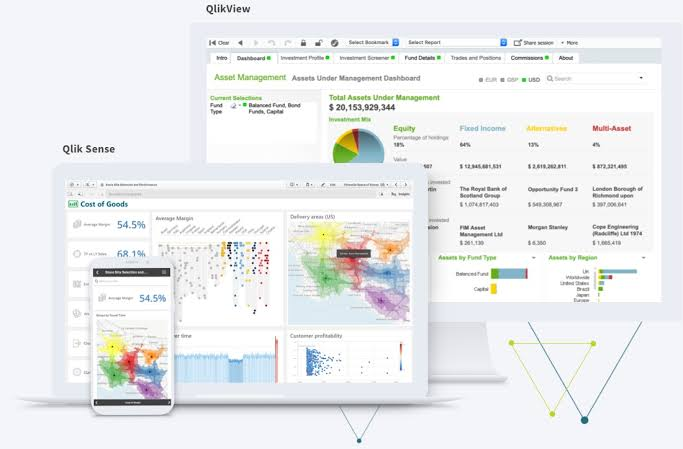
\includegraphics[scale=0.6]{imagens/qlik.jpg}
         \\{\footnotesize Fonte: (QlikView, 2019)}
         \label{exemplo qlik}
    \end{figure}
    
    Devido a facilidade para a criação de novos painéis um serviço em Qlik pode ser disponibiliza para gestores, ou seja, pessoas fora da área de TI tenham a possibilidade de acessar e criar os seus próprios painéis de visualização. 
    
\section{Fonte de dados}
    
    Com o avanço da tecnologia e da internet ,que hoje já pode ser integrado a qualquer coisa, estamos gerando cada dia mais e mais dados. Segundo pesquisas da Business Software Alliance (BSA), em 2015 o mundo gerou mais de 2,5 quintilhões de bytes por dia (2,5 quintilhões de bytes são criados todos os dias, 2015) este número está muito maior hoje em dia e a previsão é de um aumento exponencial para os próximos anos. 
    
    Toda essa quantidade de volume de dados é muito valiosa, principalmente se os dados forem tratados e analisados corretamente. Durante anos, instituições como IBGE (IBGE, 2019), Oswaldo Cruz (FIOCRUZ, 2019), Cruz vermelha (CRUZ VERMELHA, 2019), Ministério da Saúde (MINISTÉRIO DA SAÚDE, 2019) entre outros, prestam um grande serviço realizando pesquisas relacionadas a área de saúde e disponibilizando essas informações publicamente, ou seja, qualquer pessoa pode ter acesso a essas pesquisas. 
     
     A grande questão a ser discutida é se esse grande volume de dados disponível hoje está sendo utilizado de forma eficiente. Em relação a área de saúde, existem no Brasil duas principais fontes de informação, o Portal Brasileira de Dados Aberto, (Portal Brasileiro de Dados Aberto, 2019) e o portal DATASUS (DATASUS - Portal de Dados da Saúde, 2019), ambos foram utilizados como fontes de dados e pesquisas para este projeto.
    
\subsection{Portal Brasileiro de Dados Abertos}
   
    O Portal Brasileiro de Dados Abertos é um grande catálogo federado de fontes de dados abertos de temáticas diversas. 
    
    As instituições como IBGE, FIOCRUZ, Cruz Vermelha e entre outras publicam suas pesquisas na plataforma seguindo um cronograma pré estabelecido. (Sobre o dados.gov.br, 2019).
    
    O portal teve o seu primeiro ciclo de desenvolvimento entre 2011 e 2012, terminando na publicação do portal. O projeto foi feito com a participação popular, com isso, qualquer pessoa poderia participar desse projeto. O portal ainda é mantido pelo governo e vem sendo uma grande fonte de pesquisa principalmente no meio acadêmico e científico (Processo de participação social do INDA, 2019). Dentro do portal brasileiro de dados abertos é possível encontrar pesquisas de diferentes instituições em diferentes áreas, desde dados referentes a saúde, foco desse trabalho, a dados demográficos, sociais, econômicos, ambientais e etc. 
    
    Do portal brasileiro de dados aberto foram extraídas duas pesquisas desenvolvidas pelo IBGE, uma mostrando o número total de unidades básicas de saúde em funcionamento e outra apresentando o número de unidades básicas de saúde em construção em cada cidade do Brasil. 
    
\subsection{DATASUS}

    O DataSUS, ou departamento de informática do sistema único de saúde, foi criado em 1991 através da Fundação Nacional de Saúde (Funasa) e tem como objetivo fornecer a todo o sistema único de saúde suporte tecnológico, informatizando os processo e fornecendo ferramentas para o Ministério da Saúde visando melhorar o sistema único de saúde (O DATASUS, 2019). Dentro do portal do DataSUS podemos encontrar relatório sobre os softwares desenvolvidos e mantidos pelo departamento de informação do SUS, dados sobre as metodologias aplicadas, normas e regras. Os dados são exibidos em um formato de tabulação TABNET e exportado em TABWIN, esses formatos foram desenvolvidos pelo Datasus como uma forma de padronizar a apresentação dos dados. 
    
    Deste portal foi retirado três arquivos para o trabalho, estes dados apresenta o número de casos de malária, o número de casos de tuberculose e o número de doses de vacinas aplicadas em cada cidade do Brasil. 
    

\chapter{Desenvolvimento}
    
    O Desenvolvimento desse trabalho foi dividido em 6 partes conforme demonstrado na Figura \ref{etapas tcc}. Antes do início do desenvolvimento desse trabalho foi necessário realizar um estudo sobre o sistema único de saúde, que auxiliou a definir melhor os objetivos do projeto. 
    
    \begin{figure}[H]
         \centering
         \caption{Etapas do desenvolvimento}
         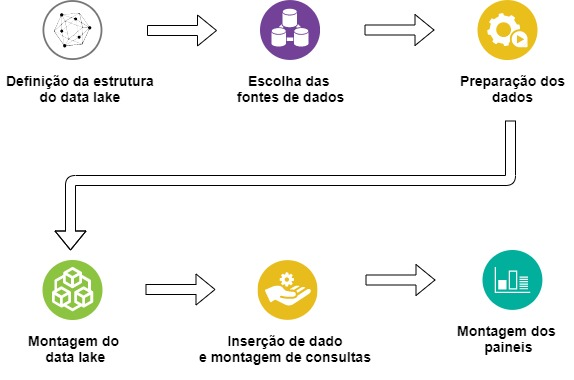
\includegraphics[scale=0.6]{imagens/etapas-tcc.jpg}
         \\{\footnotesize Fonte: Produção do próprio autor utilizando a plataforma Draw.io}
         \label{etapas tcc}
    \end{figure}
    
\section{Estudo e definição da estrutura de \textit{data lake}}

    O \textit{data lake} é um conceito, ou seja, não há um guia definitivo de como se criar um \textit{data lake} e nem há um conjunto de tecnologias específicas para se criar um \textit{data lake}, pois para cada necessidade e ambiente pode ser criado um estrutura diferente e específica. 
    
    Como o objetivo desse projeto é propor uma ideia de solução viável a alguns problemas gerenciais do SUS, adotou-se uma estrutura de \textit{data lake} simples, com poucas camadas a nós, mas que fosse possível demonstrar os resultados desejados. 
    
    Nesta etapa do desenvolvimento foi necessário pesquisar algumas ferramentas que poderiam compor, em algum nível, a estrutura do \textit{data lake} proposto neste trabalho. Como por exemplo, Microsoft Azure Data Lake Analytics (Azure Data Lake Analytics, 2019), AWS \textit{data lake} And Analytics (\textit{data lake} and Analytics on AWS, 2019), Apache Hadoop (Apache Hadoop, 2019), Google Cloud DataProc (Google Cloud DataProc, 2019), Google Cloud BigQuery (Google Cloud BigQuery, 2019) entre outros. 
    
    Depois de experimentar algumas ferramentas e estudar alguns casos de uso, como por exemplo a estrutura de \textit{data lake} construída pela empresa Movile (Grupo Movile - Ecossistema de Tecnologia Líder na América Latina, 2019) que foi apresentado no dia 26 de Setembro de 2017 no GDG Campinas - Data Fest (A jornada para implementação de um Data Lake, 2017), foi escolhido para utilização nesse trabalho a linguagem Python para o tratamento dos dados, o Dremio, uma plataforma DaaS que permite a agregação de diversas fontes de dados de formatos diferentes e uma ferramenta de consulta via SQL e o Qlik, para criação de painéis gráficos para análise de dados.
    
\section{Estudo e escolha das fontes de dados}

    A escolha dos dados que entraram na estrutura de \textit{data lake} foi uma parte essencial desse trabalho. Apesar do \textit{data lake} aceitar qualquer tipo de dados, não é recomendado que seja inseridos fontes de dados que não foram previamente analisadas, pois se for inserido dados no \textit{data lake} que não agregam valor ao negocio, isso tornaria nosso lago de dados em um pântano, ou \textit{data swamp}. 
    
    \textit{Data swamp} é um termo utilizado para definir estruturas de \textit{data lake} que foram mal projetas ou mantidas e que possuem dados incoerentes, inúteis ou não analisados e categorizados. Durante esta etapa foram encontrados algumas pesquisas, fontes de dados, que não puderam ser utilizadas dentro da estrutura de \textit{data lake} deste trabalho por não estarem atualizadas ou não serem relevantes para análise. Um exemplo são os dados do sistema de cadastramento e acompanhamento de hipertensos e diabéticos, disponível no portal do DATASUS (DATASUS - SISTEMA DE CADASTRAMENTO E ACOMPANHAMENTO DE HIPERTENSOS E DIABÉTICOS, 2019). Este banco de dados só possui informações até o mês de Abril de 2013, com isso a inserção de tal pesquisa no \textit{data lake} não agregaria, pois o ano base escolhida para o trabalho foi 2018.
    
    Esta etapa foi uma das onerosas do projeto, pois cada possível fonte de dados precisou ser analisada quanto a sua relevância para a resolução do problema proposto e a coerência dos dados contidos nela. Foi selecionado 5 pesquisas além de uma base de dados relacional contendo todas as cidades brasileiras e sua relação com estado e região. As fontes de dados utilizadas foram:
    
    \begin{description}[font=$\bullet$~\normalfont\scshape\color{black!50!black}]
    \item [UBS Existente] pesquisa do IBGE disponível no portal brasileiro de dados aberto que apresenta o número de unidades básicas de saúde por município (Distribuição Unidades Básicas de Saúde em Funcionamento - UBS. 2018);
    \item [UBS Construção] outra pesquisa extraída do portal brasileiro de dados abertas onde o IBGE disponibilizá o número de unidades básicas de saúde que estavam em construção no ano de 2018 (Número de Unidades Básicas de Saúde em Construção - UBS, 2018). 
    \item [Casos Turbeculose] dado disponível no portal do DATASUS que mostra o número de casos confirmados de turbeculose por município (TUBERCULOSE - CASOS CONFIRMADOS NOTIFICADOS NO SISTEMA DE INFORMAÇÃO DE AGRAVOS DE NOTIFICAÇÃO - BRASIL. 2019).
    \item [Casos Malária] dado contendo os registro do número de casos de malária confirmados no ano de 2018. Este dado está disponível no portal do DATASUS (MALÁRIA - CASOS CONFIRMADOS NOTIFICADOS NO SISTEMA DE INFORMAÇÃO DE AGRAVOS DE NOTIFICAÇÃO - BRASIL, 2019).
    \item [Imunizações - Doses Aplicadas] fonte de dados disponível no portal do DATASUS que contém o número de doses de vacinas aplicadas por cidade no ano de 2018 (IMUNIZAÇÕES - DOSES APLICADAS - BRASIL, 2019).
    \end{description}
    
    
\section{Preparação dos dados}
    
    Após selecionadas as fontes de dados que serão utilizadas, foi necessário utilizar scripts desenvolvidos com a linguagem de programação python para preparar os dados, pois algumas pesquisas possuíam informações irrelevantes ou repetitivas.
    
    Foi necessário abrir cada fonte de dados, entender as informações ali dispostas e definir o que necessitava ser tratado baseado no problema proposto.
    Também foi necessário padronizar a codificação dos caracteres das informações distrativas das fontes de dados, visando melhorar a leitura e possibilitar utilizar essas informações para relacionar tal fonte de dados a outra. Também foi necessário alinhar nomes de colunas. Este processo demandou um tempo significativo, pois cada fonte de dados possuía suas particularidades e com isso foi necessário adaptar o script desenvolvido para cada caso.
    
    Foram utilizados scripts que tinham como fluxo padrão ler o arquivo da pesquisa, realizar as formatações e tratamentos desejados e em seguida gravar um novo arquivo com os dados tratados. Em estrutura de \textit{data lake} maiores, essa etapa é automatizada não sendo necessário a interação humana nesse processo. Um exemplo de script utilizado na preparação dos dados pode ser visto no apêndice A. Este script foi utilizado para tratar os dados referente a registro de malária, ele ler o arquivo original que está em formato CSV, para cada linha desse arquivo o script trabalha principalmente sobre a coluna que armazena o nome da cidade, primeiro eliminando caracteres inválidos, como resto de código html, além disso o script separa o código de identificação da cidade do nome da cidade, pois essas informações vem na mesma coluna no arquivo original.
    
    
\section{Montagem do \textit{data lake}}

    Após testar algumas estruturas de \textit{data lake} e definir quais tecnologias seriam utilizadas, como vistos na seção 4.1, foi necessário conFigurar em um ambiente computacional todos os sistemas, ou seja, instalar o Dremio, Qlik, Python e os bancos de dados. Foi realizado alguns testes para entender e validar alguns recursos das plataformas escolhidas. Também foram feitos alguns testes de integração para verificar a conexão, principalmente do Dremio, com os demais sistemas.
    
    A estrutura final de \textit{data lake} criado para este trabalho contem 4 camadas, como visto na Figura \ref{estrura data lake}.
    
    \begin{figure}[H]
         \centering
         \caption{Estrutura do data lake}
         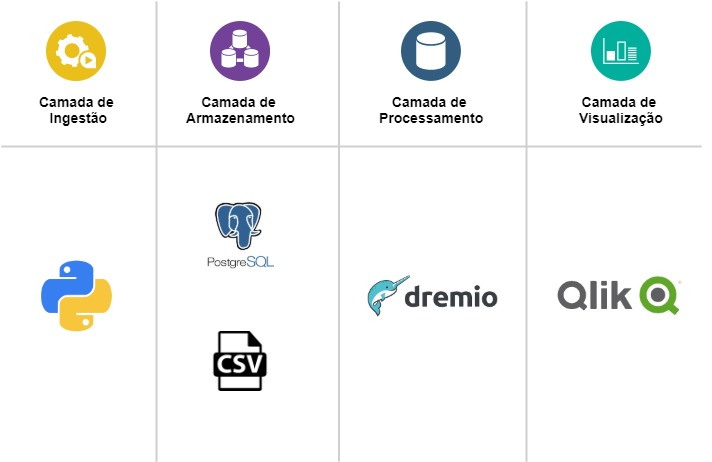
\includegraphics[scale=0.4]{imagens/meu-datalake.jpg}
         \\{\footnotesize Fonte: Produção do próprio autor feito na plataforma Draw.io}
         \label{estrura data lake}
    \end{figure}
    
    \begin{description}[font=$\bullet$~\normalfont\scshape\color{black!50!black}]
    \item [Camada de Ingestão] A camada de ingestão é responsável pelo estudo, análise, validação e preparação dos dados antes da entrada dos mesmo na estrutura de \textit{data lake}.   
    \item [Camada de Armazenamento] Na camada de armazenamento do \textit{data lake} é mantido os dados que são utilizados em nosso projeto. Este armazenamento foi feito em um ambiente local utilizando bancos de dados e arquivos hospedados localmente. 
    \item [Camada de Processamento] Na camada de processamento os dados são categorizados e indexados. Nesta camada que, utilizando os dados da camada de armazenamento, iremos relacioná-los e filtrá-los para extrair informações úteis para o negocio. 
    \item [Camada de Visualização] Nesta camada os dados preparados na camada de processamento são visualizados em forma de gráficos e relatórios interativos. 
    \end{description}

\section{Inserção dos dados e montagem das consultas no \textit{data lake}}
    
    Depois de selecionar todas as fontes de dados, seção 4.2, prepará-los na seção 4.3, e montar a estrutura de \textit{data lake}, seção 4.4, os dados foram inseridos na estrutura de \textit{data lake} montada. Após inserir os dados, foi necessário montar as consultas SQL que retornaria os dados do nosso \textit{data lake} de forma consolidada para que esses dados pudessem ser utilizados para criação de gráficos e relatórios. Durante a inserção dos dados na estrutura de \textit{data lake} foi necessário reprocessar algumas fontes de dados para alinhar e conseguir relacionar os dados da melhor forma.
    
    \begin{figure}[H]
         \centering
         \caption{Query montada no \textit{data lake}}
         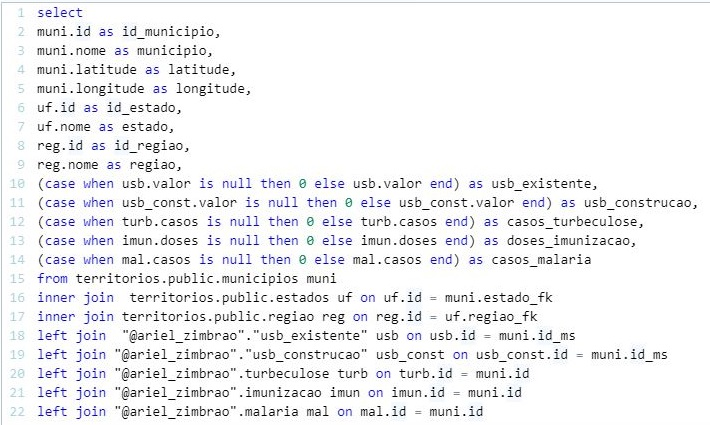
\includegraphics[scale=1.1]{imagens/query.JPG}
         \\{\footnotesize Fonte: Produção do próprio autor feito na plataforma Draw.io}
         \label{estrura data lake}
    \end{figure}
    
\section{Montagem dos painéis}
    
    Após montar a consulta, foi utilizado o recurso do Dremio que permite importar os dados para o projeto no Qlik. Esta integração deu a possibilidade de acessarmos os dados extraídos do \textit{data lake} na plataforma Qlik. 
    
    A utilização do Qlik permitiu a criação de gráficos relacionando os dados extraídos das fontes de dados selecionadas. Para este projeto foi desenvolvido um painel que permite ao usuário pesquisar e consultar os dados de número de casos registrados de tuberculose e malária, o número de vacinas aplicadas e o número de UBS (Unidades básicas de saúde) em funcionamento e construção no ano de 2018 para região, estado ou município.
    
    \begin{figure}[H]
         \centering
         \caption{Painel de análise Qlik}
         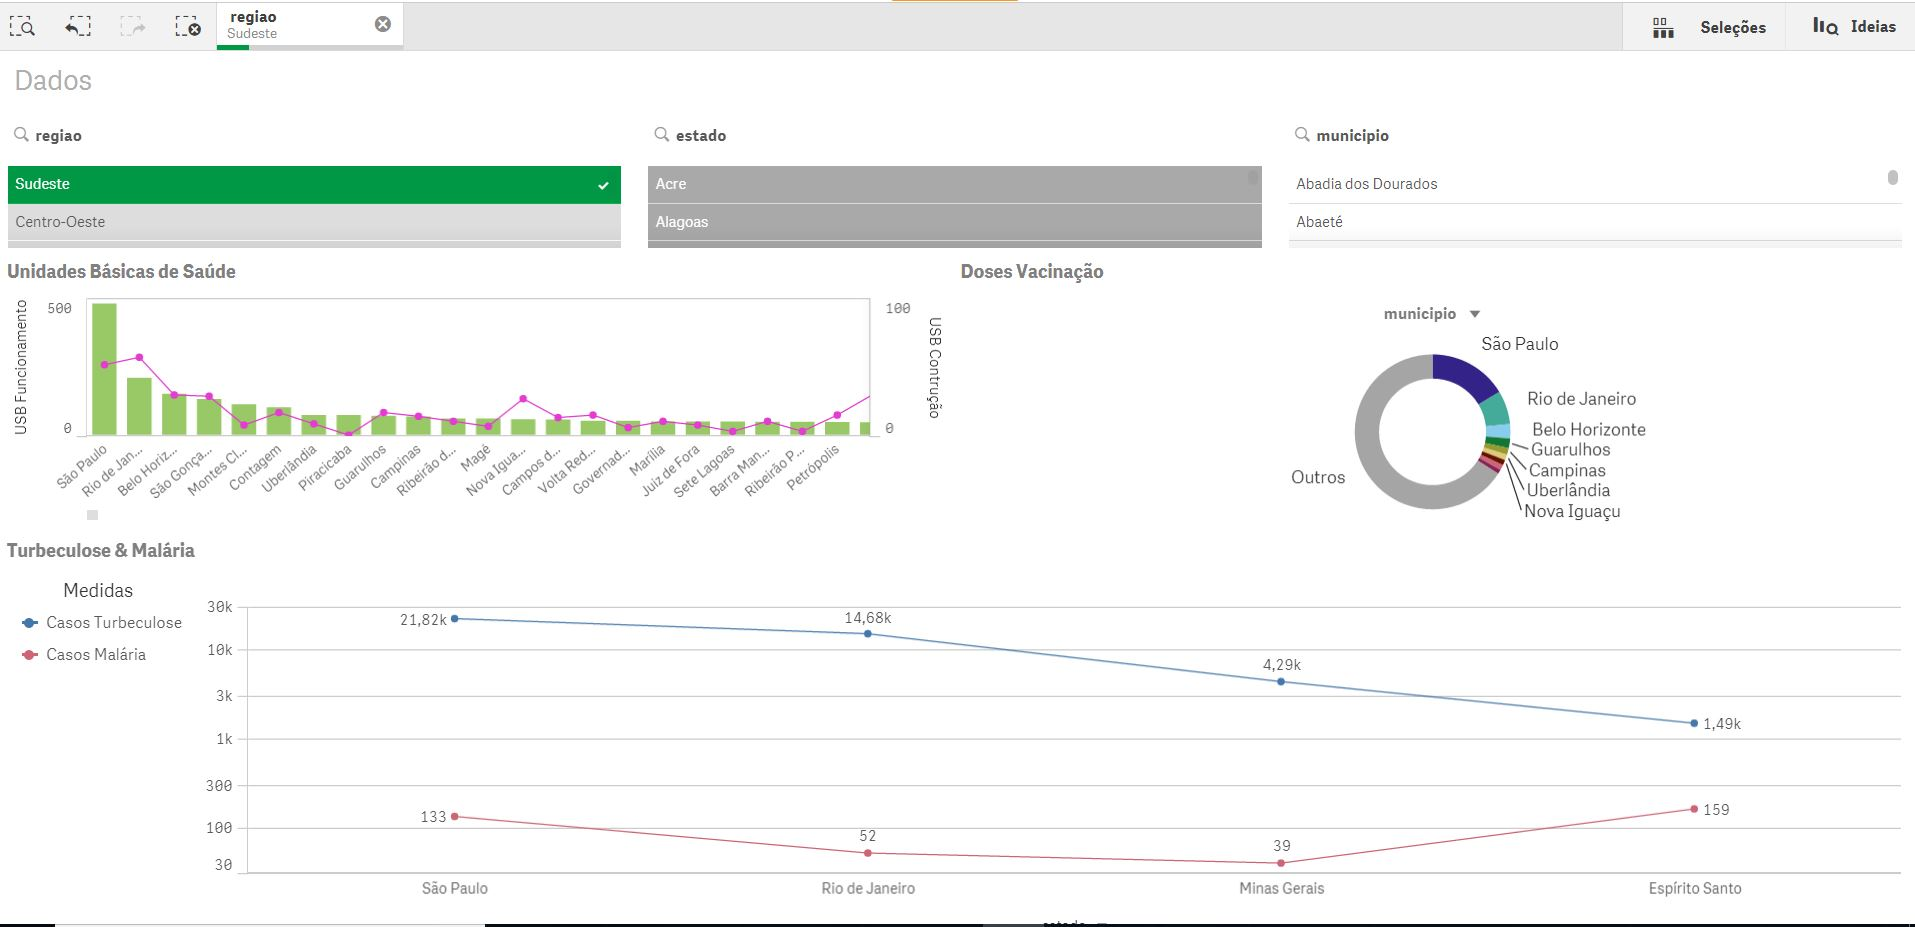
\includegraphics[scale=0.4]{imagens/paneil-total.JPG}
         \\{\footnotesize Fonte: Produção do próprio autor}
         \label{painel qlik}
    \end{figure}
    
    Com esse gráfico podemos fazer o relacionamento de informações que não estavam relacionados em suas fontes primárias, como por exemplo, podemos relacionar o número de doses de vacinas aplicadas com o número de casos confirmados de tuberculose, ou o número de postos de unidade básica de saúde com o número de casos de malária. Estes dados podem ser visto em diferentes níveis, sendo eles regional, estadual ou municipal. 
    
    O painel criado, conforme apresentado na Figura \ref{painel qlik}, é apenas uma das diversas formas que há para se organizar os dados. O objetivo dos gráfico é apresentar os dados, antes confuso e de difícil análise de uma forma mais amigável ao usuário final. Com isso conseguimos realizar a analise que foi proposta na introdução desse trabalho que é a comparação do número de unidades básicas de saúde com o número de casos registrados de turbeculose.
    
    No painel criado temos 3 gráficos. O primeiro, que pode ser visto na Figura \ref{painel usb}, apresenta o número de unidades básicas de saúde que estão em funcionamento e em construção, isso possibilita ao gestor avaliar se esse número de estabelecimento de saúde básica são o suficiente para o atendimento a população de um determinado município, estado ou região. O segundo gráfico, que pode ser visto na Figura \ref{painel vacina}, mostra o número de doses de vacinas aplicadas no ano de 2018, esse dados, unido a dados de registros de saúde pode ser utilizado para avaliar a eficiência das campanhas de vacinações. O terceiro gráfico pode ser visto na Figura \ref{painel doenca} e apresenta o número de casos confirmados de tuberculose e malária por estado ou município, esse dados e vital por pode, por exemplo, precipitar um surto de uma doença e possibilitar uma ação preventiva ou campanhas de conscientização.  
    
    \begin{figure}[H]
         \centering
         \caption{Gráfico de unidades básicas de saúde}
         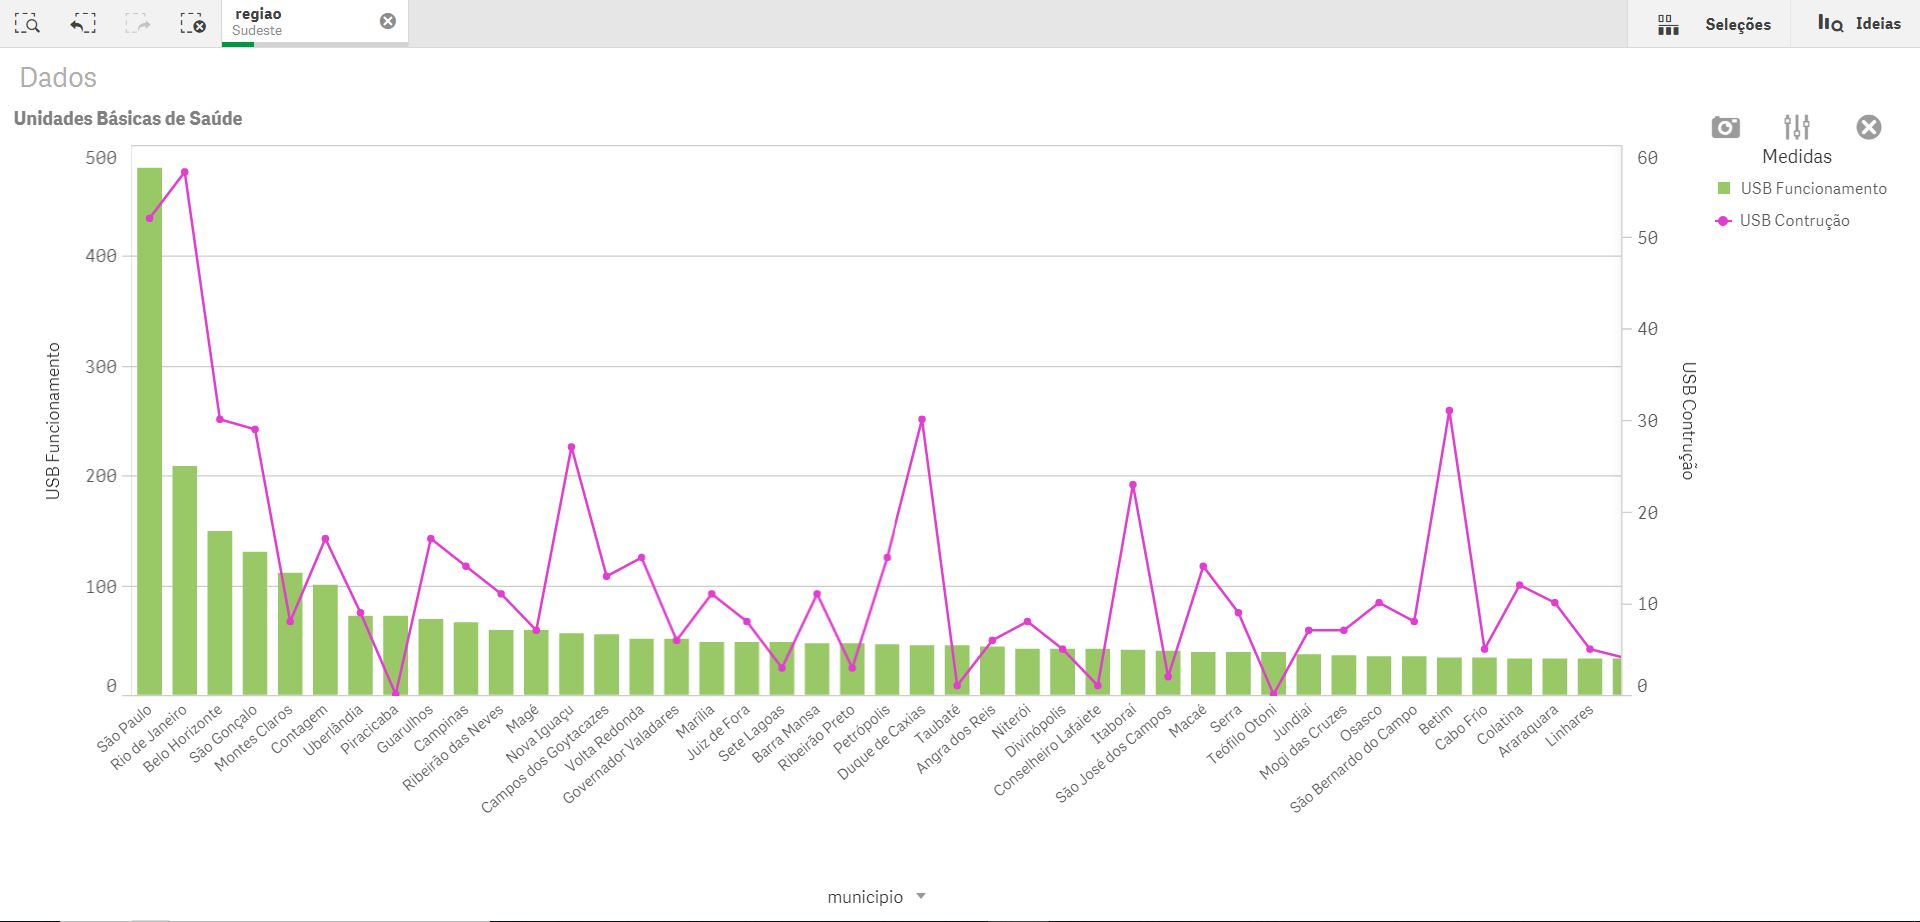
\includegraphics[scale=0.4]{imagens/painel-usb.JPG}
         \\{\footnotesize Fonte: Produção do próprio autor}
         \label{painel usb}
    \end{figure}
    
    \begin{figure}[H]
         \centering
         \caption{Gráfico de doses de vacinas aplicadas}
         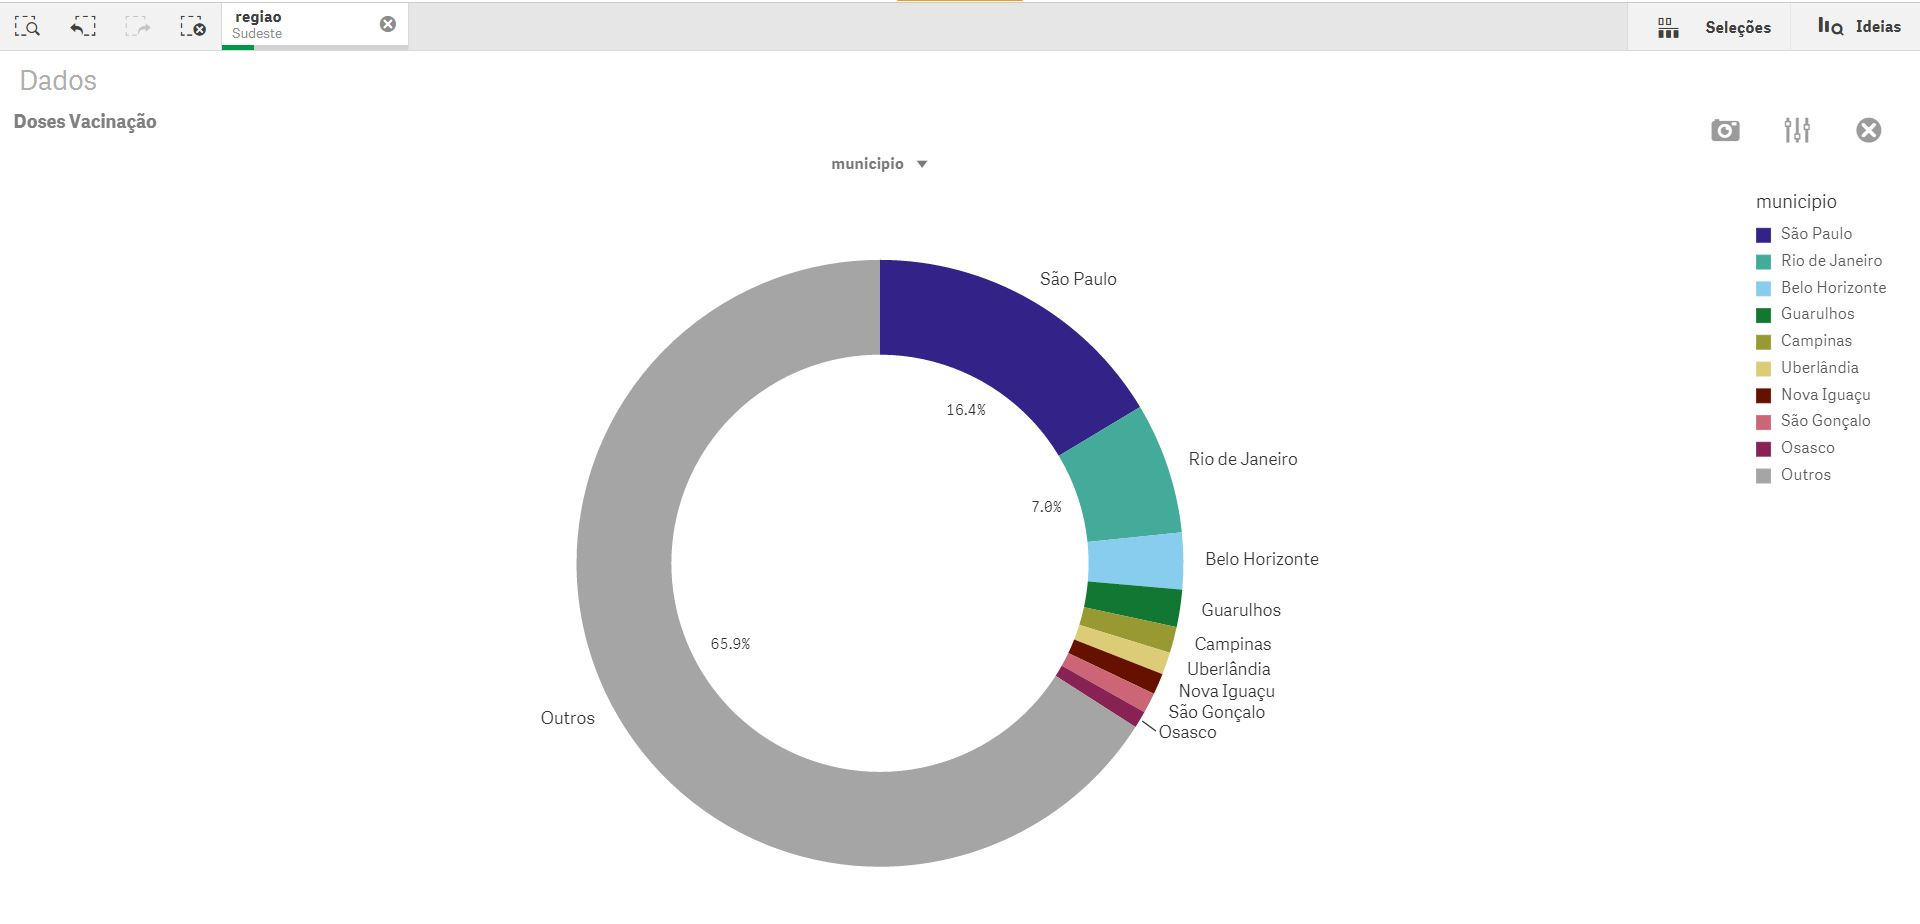
\includegraphics[scale=0.4]{imagens/painel-vacinacao.JPG}
         \\{\footnotesize Fonte: Produção do próprio autor}
         \label{painel vacina}
    \end{figure}
    
    \begin{figure}[H]
         \centering
         \caption{Gráfico de casos de turbeculose e malária}
         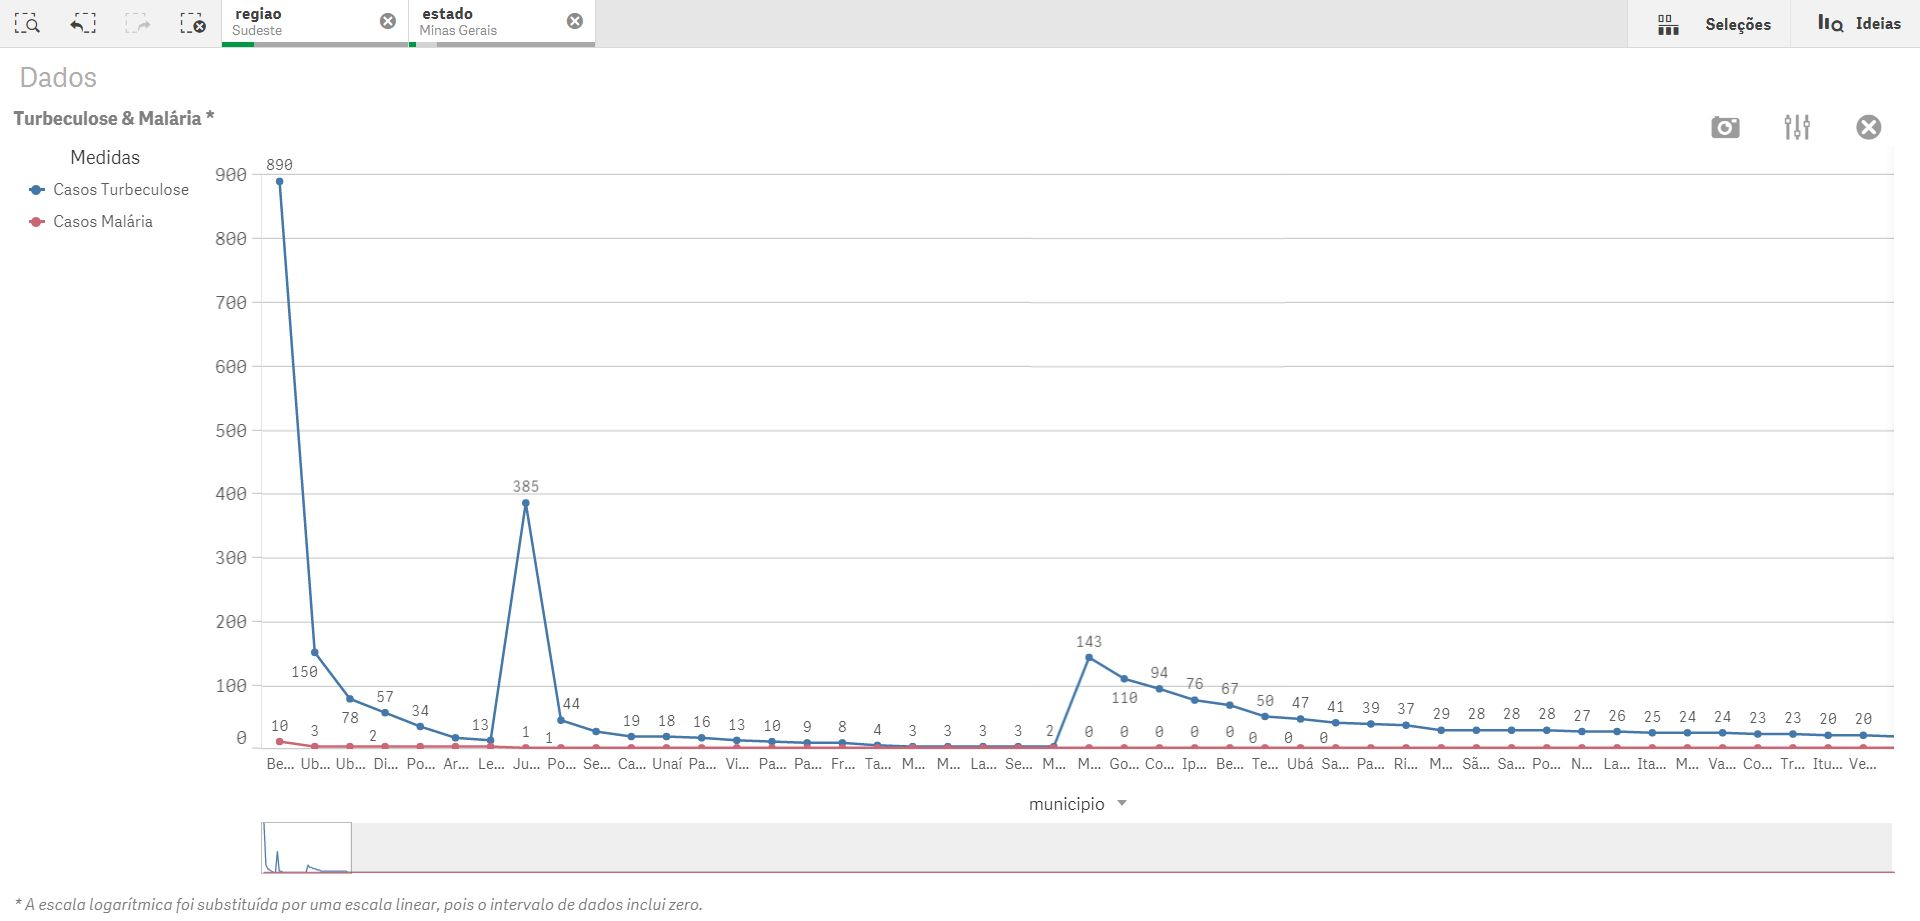
\includegraphics[scale=0.4]{imagens/painel-doenca.JPG}
         \\{\footnotesize Fonte: Produção do próprio autor}
         \label{painel doenca}
    \end{figure}
    
% ----------------------------------------------------------
% Considerações Finais
% ----------------------------------------------------------
\chapter{Conclusão}
    
    Com este trabalho podemos verificar que a utilização de uma estrutura de data lake é uma solução viável para realizar análises de dados públicos, não somente na área de saúde, mas tal tecnologia pode ser aplicada sobre qualquer temática. Uma das principais dificuldades na criação e manutenção de um \textit{data lake}, que foi encontrado durante o desenvolvimento desse trabalho, foi selecionar e preparar os dados mantendo a coerência de toda a estrutura, ou seja, a etapa mais onerosa do desenvolvimento deste projeto foi selecionar os dados que entrariam no \textit{data lake} para que, semanticamente, uma análise unificada desses dados fosse útil.
    
    No painel que desenvolvemos já conseguimos realizar consultas que relacionem dados do Ministério da Saúde com dados do IBGE, buscando encontrar relações entre eles. Essas informações podem ser utilizadas por um gestor para auxilio a tomada de decisão, tornando, por exemplo, a distribuição de verbas mais efetiva. 
    
    Algumas outras abordagens podem ser desenvolvidas a partir dos mesmos princípios que deram origem a este trabalho, agregando mais dados e dando mais possibilidades de analise, como por exemplo. 

    \begin{description}[font=$\bullet$~\normalfont\scshape\color{black!50!black}]
    
    \item [Ampliação do \textit{data lake}] Ainda há muitos dados que podem ser inseridos no \textit{data lake} apresentado nesse trabalho, a inserção desses dados aumentaria as possibilidades de analise. Informações como registro de doenças infeciosas, numero de população por município, ou até mesmo seria possível realizar a interação com redes sociais para coletar a opinião online da população.
    
    \item [Automação do \textit{data lake}] A solução de \textit{data lake} apresentada neste trabalho apresenta um estrutura simples em relação a complexidade que uma estrutura de tal tecnologia é capaz de ter. Um possível trabalho futuro é a ampliação do \textit{data lake} apresentado nesse trabalho, implementando a automatização de processos como por exemplo, a criação de camadas de software que possibilite a inserção por parte de um usuário, de novos dados. Também é possível publicar a plataforma do Qlik online, possibilitando que qualquer pessoa visualize os painéis desenvolvido e também crie os seus próprios relatórios com os dados disponíveis no \textit{data lake}.
    
    \item [Inserção de modulos de inteligência artificial (IA) no \textit{data lake}] Tendo em vista que temos em um \textit{data lake} é possível e extremamente interessante a inserção de módulos de IA em nosso \textit{data lake}, com o objetivo, por exemplo identificar padrões nos dados e dar sugestões de ações.
    
    \item [Criação de serviço integrado] Uma outra solução é criar um serviço para armazenar e integrar os dados. Tal aplicação pode ser um serviço web que receba dos demais sistemas de gestão de saúde pública dados e apresente eles em painéis gráficos. Com esse serviço os softwares de gestão publica de saúde poderiam enviar periodicamente os dados 
    
    \end{description}
% ----------------------------------------------------------
% ELEMENTOS PÓS-TEXTUAIS
% ----------------------------------------------------------
\postextual
% ----------------------------------------------------------

% ----------------------------------------------------------
% Referências bibliográficas
% ----------------------------------------------------------
% bibliografia
\bibliographystyle{plain}
\bibliography{bibliografia.bib}
% ---

2,5 QUINTILHÕES DE BYTES SÃO CRIADOS TODOS OS DIAS. Disponivel em <https://cio.com.br/tome-nota-2-5-quintilhoes-de-bytes-sao-criados-todos-os-dias/>. Acessado em <01/11/2019>

A. Dziedzic & A. J. Elmore, 2015. Data Transformation and Migration in Polystores. MIT Computer Science & Artificial Intelligence Lab. Disponivél em <https://adam-dziedzic.github.io/static/assets/papers/dziedzic_hpec16_data_migration.pdf>. Acesso em 22/10/2019

A JORNADA PARA IMPLEMENTAÇÃO DE UM DATA LAKE. Disponivel em <https://www.infoq.com/br/presentations/a-jornada-para-implementacao-de-um-data-lake/>. Acessado em <20/10/2019>

ABOUT PYTHON. Disponivel em <https://www.python.org/about/>. Acessado em <27/10/2019>

AMAZON ATHENA. PAGINA INICIAL. Disponivel em <https://aws.amazon.com/pt/athena/>. Acessado em <28/10/2019>

AMAZON REDSHIFT. PAGINA INICIAL. Disponivel em <https://aws.amazon.com/pt/redshift/>. Acessado em <28/10/2019>

AMAZON S3. PAGINA INICIAL. Disponivel em <https://aws.amazon.com/pt/s3/>. Acessado em <28/10/2019>

ANÁLISE DE DADOS PARA O BUSINESS INTELLIGENCE MODERNO. PAGINA INICIAL. Disponivel em <https://www.qlik.com/pt-br>. Acessado em <12/10/2019>

APACHE HADOOP. PAGINA INICIAL. Disponivel em <https://hadoop.apache.org/>. Acessado em <27/10/2019>

AWS - AMAZON WEB SERVICE. PAGINA INICIAL. Disponivel em <https://aws.amazon.com/pt/>. Acessado em <07/10/2019>

AWS - WHAT IS A DATA LAKE. Disponivel em <https://aws.amazon.com/big-data/data lakes-and-analytics/what-is-a-data-lake/>. Acessado em <07/10/2019>

AZURE DATA LAKE ANALYTICS. PAGINA INICIAL. Disponivel em <https://azure.microsoft.com/pt-br/solutions/data-lake/>. Acessado em <27/10/2019>

BANCO DE DADOS - ORACLE. PAGINA INICIAL. Disponivel em <https://www.oracle.com/br/database/>. Acessado em <28/10/2019>

CONVERGÊNCIA DIGITAL, GLOBALWEB DESENVOLVE DATA LAKE PARA A HEALTHTECH. NOVEMBRO DE 2018. Disponivel em <http://www.convergenciadigital.com.br/cgi/cgilua.exe/sys/start.htm?UserActiveTemplate=site&infoid=49542&sid=97>. Acessado em <28/10/2019>

CRUZ VERMELHA. CRUZ VERMELHA BRASILEIRA. PÁGINA INICIAL. Disponivel em <http://www.cruzvermelha.org.br/en/>. Acessado em <29/09/2019>

DATA LAKE AND ANALYTICS ON AWS. PAGINA INICIAL. Disponivel em <https://aws.amazon.com/pt/big-data/data lakes-and-analytics/>. Acessado em <27/10/2019>

DATASUS - PORTAL DE DADOS DA SAÚDE. PAGINA INICIAL. Disponivel em <http://www2.datasus.gov.br/DATASUS/index.php>. Acessado em <20/10/2019>

DATASUS - SISTEMA DE CADASTRAMENTO E ACOMPANHAMENTO DE HIPERTENSOS E DIABÉTICOS. Disponivel em <http://tabnet.datasus.gov.br/cgi/deftohtm.exe?hiperdia/cnv/hdRJ.def>. Acessado em <28/10/2019>

DISTRIBUIÇÃO UNIDADES BÁSICAS DE SAÚDE EM FUNCIONAMENTO - UBS. Disponivel em <http://dados.gov.br/dataset/ubs_funcionamento>. Acessado em <08/11/2019>

DREMIO IS THE DATA LAKE ENGINE, PAGINA INICIAL. Disponivel em <https://www.dremio.com>. Acessado em <12/10/2019>

FIOCRUZ. FUNDAÇÃO OSWALDO CRUZ . PÁGINA INICIAL. Disponivel em <https://portal.fiocruz.br/>. Acessado em <29/09/2019>

FUNCIONAL HEALTH TECH. PAGINA INICIAL. Disponivel em <https://www.funcionalcorp.com.br/>. Acessado em <28/10/2019>

GLOBALWEB - UMA NUVEM DE SOLUÇÕES PARA SUA EMPRESA. PAGINA INICIAL. Disponivel em <https://www.globalweb.com.br>. Acessado em <28/10/2019>

GOOGLE CLOUD BIGQUERY. PAGINA INICIAL. Disponivel em <https://cloud.google.com/bigquery/?hl=pt-br>. Acessado em <27/10/2019>

GOOGLE CLOUD DATAPROC. PAGINA INICIAL. Disponivel em <https://cloud.google.com/dataproc/?hl=pt-br>. Acessado em <27/10/2019>

GOOGLE CLOUD STORAGE. PAGINA INICIAL. Disponivel em <https://cloud.google.com/storage/>. Acessado em <28/10/2019>

GOOGLE CLOUD. PAGINA INICIAL. Disponivel em <https://cloud.google.com/>. Acessado em <07/10/2019>

GOVDATA - PLATAFORMA DE ANÁLISE DE DADOS. PAGINA INICIAL. Disponivel em <https://www.govdata.gov.br/index.html>. Acessado em <09/12/2019>

GRAFANA - THE OPEN OBSERVABILITY PLATFORM. PAGINA INICIAL. Disponivel em <https://grafana.com/>. Acessado em <27/10/2019>

GRUPO MOVILE - ECOSSISTEMA DE TECNOLOGIA LÍDER NA AMÉRICA LATINA. PAGINA INICIAL. Disponivel em <https://www.movile.com.br/>. Acessado em <28/10/2019>

IBGE. INSTITUTO BRASILEIRO DE GEOGRAFIA E ESTATÍSTICA, PÁGINA INICIAL. Disponivel em <https://ibge.gov.br/>. Acessado em <29/09/2019>

IMUNIZAÇÕES - DOSES APLICADAS - BRASIL. Disponivel em <http://tabnet.datasus.gov.br/cgi/dhdat.exe?bd_pni/dpnibr.def>. Acessado em <16/11/2019>

INFLUXDB - PORPUSE-BUILT OPEN SOURCE TIME SERIE DATABASE. PAGINA INICIAL. Disponivel em <https://www.influxdata.com/>. Acessado em <27/10/2019>

INFLUXDB TIME SERIES DATA MONITORING WITH GRAFANA. Disponivel em <https://www.influxdata.com/blog/how-to-use-grafana-with-influxdb-to-monitor-time-series-data/>. Acessado em <28/10/2019>

INFORMATION AGE - THE DIFFERENCE BETWEEN A DATA SWAMP AND A DATA LAKE? 5 SIGNS. Disponivel em <https://www.information-age.com/data-swamp-data-lake-123481597/>. Acessado em <07/10/2019>

ISTOÉ DINHEIRO, FUNCIONAL HEALTH TECH INVESTE EM BIG DATA PARA A SAÚDE, JUNHO DE 2019. Disponivel em <https://www.istoedinheiro.com.br/funcional-healh-tech-investe-em-big-data-para-a-saude/>. Acessado em <28/10/2019>

LEGISLAÇÃO DO SUS. PRINCÍPIOS DO SUS (SISTEMA ÚNICO DE SAÚDE). Disponivel em <http://www.legislacaodosus.com.br/blog/principios-do-sus-sistema-unico-de-saude>. Acessado em <01/10/2019>

MALÁRIA - CASOS CONFIRMADOS NOTIFICADOS NO SISTEMA DE INFORMAÇÃO DE AGRAVOS DE NOTIFICAÇÃO - BRASIL. Disponivel em <http://tabnet.datasus.gov.br/cgi/deftohtm.exe?sinannet/cnv/malabr.def>. Acessado em <16/11/2019>

MINISTÉRIO DA SAÚDE. O SUS. Disponivel em <http://http://www.saude.gov.br/sistema-unico-de-saude>. Acessado em <29/09/2019>

MINISTÉRIO DA SAÚDE. O SUS.  PÁGINA INICIAL. Disponivel em <http://http://www.saude.gov.br/>. Acessado em <29/09/2019>

MINISTÉRIO DA SAÚDE. PRINCÍPIOS DO SUS. Disponivel em <http://www.saude.gov.br/sistema-unico-de-saude/principios-do-sus>. Acessado em <09/09/2019>

MINISTÉRIO DA SAÚDE, SECRETARIA DE GESTÃO ESTRATÉGICA E, PARTICIPATIVA – SGEP, COMITÊ GESTOR DO DECRETO 7508 – GE COAP. Contrato Organizativo de Ação Pública da Saúde. Brasília, 2011.

MONGODB - THE MOST POPULAR DATABASE FOR MORDEN APPS. PAGINA INICIAL. Disponivel em <https://www.mongodb.com/>. Acessado em <28/10/2019>

MONGODB CRUD OPERATIONS - MONGODB MANUAL. Disponivel em <https://docs.mongodb.com/manual/crud/>. Acessado em <28/10/2019>

MOVILE - O GRUPO. Disponivel em <https://www.movile.com.br/o-grupo>. Acessado em <28/10/2019>

MV INFORMATIZA SISTEMA DE SAÚDE PÚBLICA DO PARANA. Disponivel em <http://www.mv.com.br/pt/solucoes/saude-publica>. Acessado em <01/11/2019>

NÚMERO DE UNIDADES BÁSICAS DE SAÚDE EM CONSTRUÇÃO - UBS. Disponivel em <http://dados.gov.br/dataset/ubs_construcao>. Acessado em <08/11/2019>

O DATASUS. Disponivel em <http://datasus.saude.gov.br/datasus>. Acessado em <01/11/2019>

PERNAMBUCO, SECRETARIA ESTADUAL DE SAÚDE, SECRETARIA EXECUTIVA DE COORDENAÇÃO GERAL, DIRETORIA GERAL DE PLANEJAMENTO. Nota Técnica Nº 06 - Orientações COAP. Estado de Pernambuco, 2013.

PLATAFORMA DE DADOS DA MICROSOFT. PAGINA INICIAL. Disponivel em <https://www.microsoft.com/pt-br/sql-server>. Acessado em <12/10/2019>

PORTAL BRASILEIRO DE DADOS ABERTO, PAGINA INICIAL. Disponivel em <http://dados.gov.br/>. Acessado em <20/10/2019>

POSTGRESQL. PAGINA INICIAL. Disponivel em <https://www.postgresql.org/>. Acessado em <28/10/2019>

PRESTO - DISTRIBUTED SQL QUERY ENGINE FOR BIG DATA. PAGINA INICIAL. Disponivel em <http://prestodb.github.io/>. Acessado em <28/10/2019>

PROCESSO DE PARTICIPAÇÃO SOCIAL DO INDA. Disponivel em <http://dados.gov.br/pagina/processo-de-participacao-social-da-inda>. Acessado em <01/11/2019>

PYTHON MANTÉN ASCENÇÃO E GANHA AINDA MAIS POPULARIDADE. Disponivel em <https://computerworld.com.br/2019/01/08/python-mantem-ascensao-e-ganha-ainda-mais-popularidade/>. Acessado em <06/11/2019>

QLIKVIEW. PAGINA INICIAL. Disponivel em <https://www.qlik.com/pt-br/products/qlikview>. Acessado em <29/10/2019>

REDIS. PÁGINA INICIAL. Disponivel em <https://redis.io/>. Acessado em <28/10/2019>

S. Bimonte, A. Tchounikine, M. Miquel. Spatial OLAP: Open Issues and a Web Based Prototype. In: AGILE International Conference on Geographic Information Science, 10, 2007, Aalborg University, Denmark 2007.1 – 11

SOBRE O DADOS.GOV.BR. Disponivel em <http://dados.gov.br/pagina/sobre>. Acessado em <01/11/2019>

SOFTWARE DE BUSSINESS INTELIGENCE PARA SAÚDE - QLIK. Disponivel em <https://www.qlik.com/pt-br/solutions/industries/healthcare>. Acessado em <30/10/2019>

SQL SERVER DATA TOOLS. Disponivel em <https://docs.microsoft.com/pt-br/sql/ssdt/sql-server-data-tools?view=sql-server-ver15>. Acessado em <28/10/2019>

TABLEAU - SOFTWARE DE ANÁLISE E BUSSINESS INTELLIGENCE. PAGINA INICIAL. Disponivel em <https://www.tableau.com/pt-br>. Acessado em <28/10/2019>

TEXAS CHILDREN'S HOSPITAL. PAGINA INICIAL. Disponivel em <https://www.texaschildrens.org/>. Acessado em <30/10/2019>

THE TECHNOLOGY OF AN OLAP CUBE. Disponivel em <https://galaktika-soft.com/blog/olap-cubes.html>. Acessado em <10/12/2019>

TUBERCULOSE - CASOS CONFIRMADOS NOTIFICADOS NO SISTEMA DE INFORMAÇÃO DE AGRAVOS DE NOTIFICAÇÃO - BRASIL. Disponivel em <http://tabnet.datasus.gov.br/cgi/tabcgi.exe?sinannet/cnv/tubercbr.def>. Acessado em <13/11/2019>

WHAT IS BUSINESS INTELLIGENCE (BI)?. Disponivel em <https://olap.com/learn-bi-olap/olap-bi-definitions/business-intelligence/>. Acessado em <12/10/2019>

WHAT IS DATABASE AS A SERVICE. Disponivel em <https://www.ibm.com/developerworks/community/blogs/8f058ee2-f3aa-4976-aeb8-4e6102dc86f8/entry/what-is-database-as-a-service-dbaas?lang=en>. Acessado em <22/10/2019>

WHY TERSONFLOW. Disponivel em <https://www.tensorflow.org/about>. Acessado em <06/11/2019>

% ----------------------------------------------------------
% Apêndices
% ----------------------------------------------------------

% ---
% Inicia os apêndices
% ---
\begin{apendicesenv}
	
	% Imprime uma página indicando o início dos apêndices
	\partapendices
	
% ----------------------------------------------------------
\chapter{Exemplo de script em python para preparação dos dados}
\begin{lstlisting}[language=Python]
import csv
import re
linhas = []

def convert(dado):
    return str(dado).replace("\"","").replace("<b>", "")
    .replace("</b>", "").replace("<i>", "").replace("</i>", "")

with open('malaria.csv') as f:
    reader = csv.reader(f, delimiter=';')
    for row in reader:
        linhas.append(row)


with open("saida.csv", 'a') as csvfile:
    writer = csv.writer(
        csvfile, 
        delimiter=',', 
        quotechar='"',
        quoting=csv.QUOTE_MINIMAL
    )
    for l in linhas:

        dado = list(map(convert, l))

        s = re.sub('[a-z]', '', dado[0].lower()).strip()
        dado[0] = re.sub('[0-9]', '', dado[0]).strip()
        numero = ''.join(i for i in s if i.isdigit())
        dado.append(numero)
        writer.writerow(dado)

\end{lstlisting}

% ----------------------------------------------------------
	
\end{apendicesenv}
% ---

% ----------------------------------------------------------
% Anexos
% ----------------------------------------------------------

% ---
% Inicia os anexos
% ---
%\begin{anexosenv}
	
	% Imprime uma página indicando o início dos anexos
	%\partanexos
	
	% ---
    %\chapter{Exemplo}
    % ---
	
%\end{anexosenv}

\end{document}
